%!TEX root = ../Main.tex

\chapter{Genetic map of \textit{Yr15} with RNA-Seq.}
\glsresetall
\chaptermark{Genetic map of \textit{Yr15}}
\label{yr15}
%This section describes in detail than the paper of \citet{Ramirez-Gonzalez-2014}
 
%Breeding importance of \textit{Yr15} and original source (an introgression of \textit{T. diccocoides}). 
\section{Background.}
Wheat breeding programs aim to improve the wheat lines available for production.
One of the traits desired in an elite line is the resistance to pathogens, such as\gls{pst}, the fungi responsible of yellow rust.
A source of resistance genes are introgressions from other species, such as \textit{Triticum dicoccoides} (emmer, Figure \ref{fig:lit:polyplody}). 
In the University of Sydney a collection of \glspl{nil} with introgressions to several yellow rust resistance genes on a susceptible background were developed \citep{Wellings1998}. 
In this chapter the \gls{nil} for the \textit{Yr15} locus is used to produce a mapping population to produce a mapping population, which when combined with mapping by sequencing approaches, results in improved diagnostic markers. 

%TODO: Paragraph explaining NILs
\subsection{Segregation on \texorpdfstring{$F_{2}$}{F2} populations.}
\label{yr15:f2}
Molecular markers can be used to select lines by testing if certain allele is present in a line, without the need to phenotype  the given line.
To find which regions are linked to a trait the use of $F_{2}$ mapping populations is a common practice, especially for major single gene traits.
The population is produced by crossing two (usually homozygous) parents ($P_1$ and $P_{2}$) with different alleles, A/A (dominant, resistant if containing \textit{Yr15}) and a/a (recessive, susceptible in our experiment).
When the trait is dominant and has a Mendelian segregation, the $F_1$ population should exhibit the dominant trait, as it has a copy of each allele (A/a). 
The $F_1$ is then self-pollinated to produce and $F_2$ population which should segregate with a ratio of 1:2:1, dominant:heterozygous:recessive respectively.
This generates a population with a phenotypic ratio of 3:1 (resistant:susceptible), since the effect of the recessive allele is masked by the dominant allele (\citealt{VanOoijen2013}; Figure \ref{fig:yr15:f2schematic}).  

\begin{figure}
  \centering
   \begin{subfigure}{0.45\textwidth}
   \caption{}
   \label{fig:yr15:f2schematic}
   \centering
   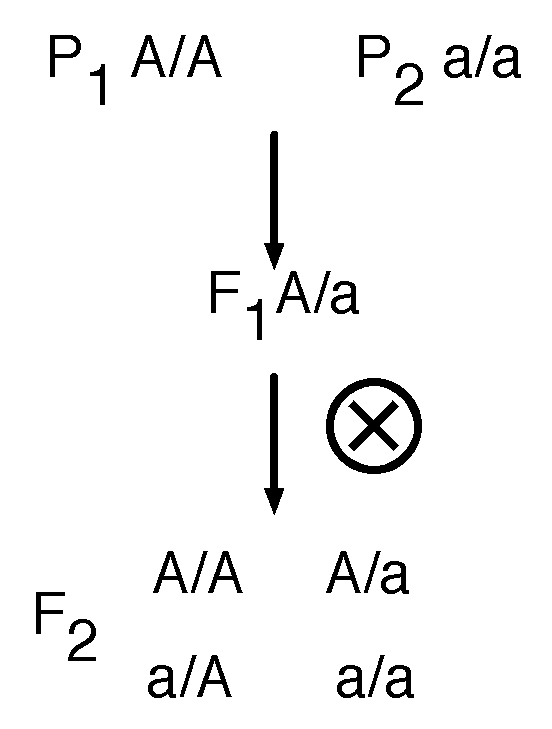
\includegraphics[height=0.3\textheight]{Yr15/Figures/population/F2schematic.pdf}
  \end{subfigure}
  ~
   \begin{subfigure}{0.5\textwidth}
   \caption{}
   \label{fig:yr15:BSAschematic}
   \centering
   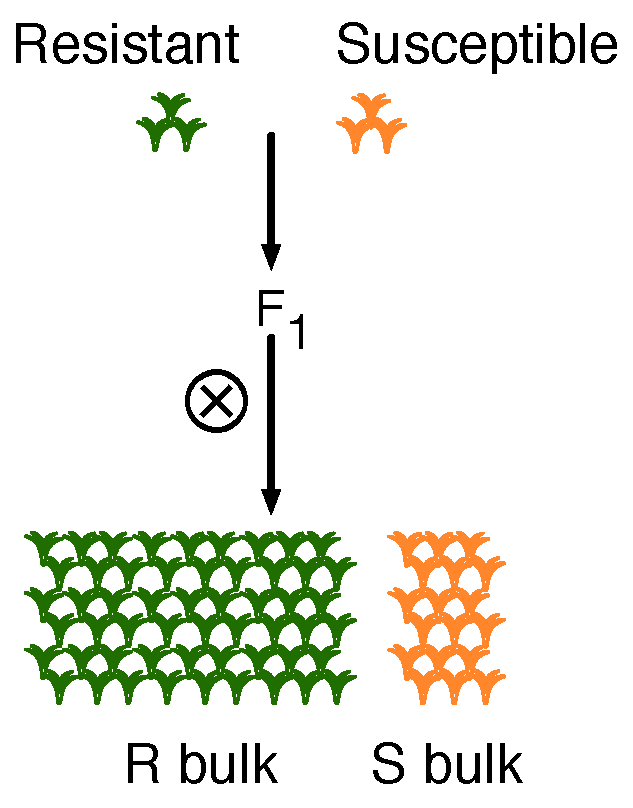
\includegraphics[height=0.3\textheight]{Yr15/Figures/BSA.pdf}
  \end{subfigure}
   \caption[Alleles on $F_2$ population and Bulk Segregant Analysis.]{Alleles on $F_2$ population and Bulk Segregant Analysis. The $\otimes$ represent self-pollination. (\subref{fig:yr15:f2schematic}) The cross of two homozygous parents, $P_{1}$ and $P_{2}$, with a dominant and a recessive allele of a gene produces an heterozygous $F_{1}$. The $F_{1}$ crossed with itself produce a segregating $F_{2}$ population with a 1:2:1 ratio (A/A:A/a:a/a). The upper and lower cases represent dominant and recessive alleles, respectively. (\subref{fig:yr15:BSAschematic}) Bulk Segregant Analysis consist on pooling DNA from the $F_{2}$ population. The DNA is mixed in bulks coming from plants with a shared phenotype. For a dominant resistance gene, an R sulk contains only resistant individuals (with A/A and A/a genotype) and, an S bulk with the susceptible individuals (with a/a genotype). } 
  
\end{figure}

\subsection{SNP calling}
\gls{bsa} consists on pooling the DNA of individuals from a segregating population with contrasting phenotypes \citep{Michelmore1991} in a segregating population. 
By combining multiple independent individuals with similar phenotypes, one can identify regions which are over-represented or enriched in the corresponding bulks. 
Regions which are not linked to the trait of interest show up as heterozygous in the bulks, whereas regions which are linked to the trait of interest will be enriched for either parental allele.
Here one would expect an enrichment of the resistant allele A with respect to the susceptible allele a in the resistant bulk. 
Analogously, one would expect the absence of the resistant allele A in the susceptible bulk (Figure \ref{fig:yr15:BSAschematic}). 
This approach can be used to identify SNPs using \gls{ngs}-based methods, such as exome capture \citep{Hodges2007}, RNA-Seq \citep{Pickrell2010}, whole genome re-sequencing \citep{Schneeberger2009}, among others. 

To find SNPs linked to the trait segregating in an $F_{2}$ population using \gls{ngs} data there are several options. 
In organisms with a contiguous reference genome, a normalised count of the times each allele is observed is enough to find the region linked to the trait; this simple ratio is called SNP-Index \citep{Takagi2013a}.
However, wheat is a polyploid organism, with an average identity between homoeologues of over 98\%. 
Because of the high identity, reads coming from different homoeologues may map to the same position; and this problem is exacerbated in cases where a reference sequence for some of the homoeologues is absent. 
The \gls{bfr} \citep{Trick2012} methodology can work on organisms that have more than one pseudo genome and where not all of the genes, either homoeologues or paralogues, have been characterised independently; it works with a single reference by collapsing similar regions. 
Both methodologies rely on an enrichment of the alleles linked to the trait in the corresponding locus. 

An example of homoeologous variants between two sub-genomes of wheat is the G$>$T variant at position 181; K in consensus (Figure \ref{fig:yr15:bfr}). This variant will produce the same ambiguity code for both parental consensus sequences and can therefore be excluded. 
An example of real allelic varietal SNPs between the parental genotypes is exemplified by the G$>$A variant at position 184; R in consensus. These variants are distinguished by the presence in only one of the consensus sequences. 
The allelic SNPs are then examined further with the alignments of the bulks to identify the SNPs that are enriched on the resistant plants.
The SNP index is the proportion of times an alternative allele is observed over the coverage at certain position, in the example the susceptible bulk has an SNP index of $1/8=0.125$ while the resistant bulk has an index of $6/8=0.75$ \citep{Takagi2013a}. 
The \glspl{bfr} are then calculated by dividing the SNP Index of the sample containing the target phenotype (resistance) over the sample without the trait (susceptible). For this example, it would be $0.75/0.125=6$.  
A high BFR suggests that the \acrshort{snp} is linked to the target trait \citep{Trick2012}. 
The implementation of the BFR analysis is detailed in Section \ref{yr15:sub:bfr} and the results on the $F_2$ population are discussed in Section \ref{sec:yr15:bfr}. 
%Repeated
%The Bulk Frequency Ratio (BFR) methodology can work on organisms that have more than one pseudo genome with not all the genes, either homoeologues or paralogues, characterised independently; it works with a single reference collapsing similar regions.

\begin{figure}
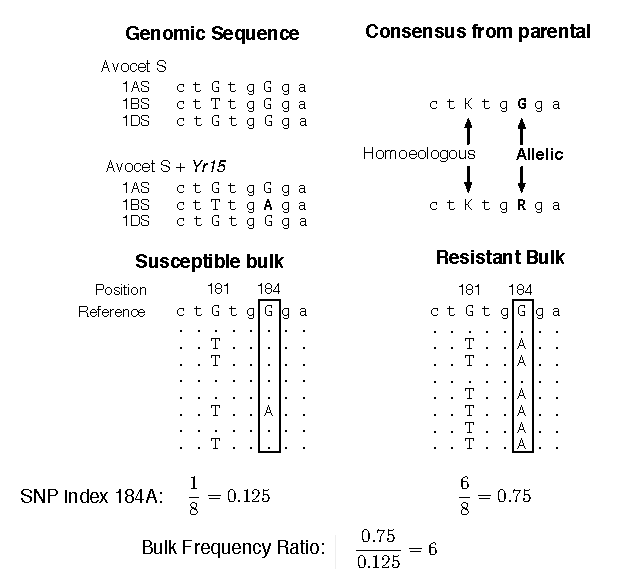
\includegraphics[width=1\textwidth]{Yr15/Figures/bfr.pdf}
\caption[BFR formula]{BFR formula. Illustration of a non-informative homoeologous SNP (G181T) present in both parental lines, and an informative allelic SNP (G184A), only present in the resistant progenitor Avocet S + Yr15. The consensus sequences from the parental genotypes include this information in the form of ambiguity codes (K and R, respectively). In the bulks, the individual reads align across the reference sequence, with matches indicated by dots, and polymorphisms at positions 181 and 184 indicated by the corresponding nucleotide variants. The SNP index is calculated as the frequency of the informative allelic SNP in each bulk. The Bulk Frequency Ratio is the quotient of the resistant and susceptible bulk SNP Indexes. Figure previously published in \citet{Ramirez-Gonzalez2015c}. }
\label{fig:yr15:bfr}
\end{figure}

To call SNPs from RNA-Seq, a reference transcriptome rather than a reference genome sequence is used as target to align the reads. 
The UniGenes database, from NCBI, contains the known genes of each species with all the variations of each gene automatically collapsed and represented with the longest available \acrshort{cdna} \citep{PontiusJUWagnerL2002}. 
The \acrshort{ucw}  gene set described in \citet{Krasileva2013} contains 94,177 models from tetraploid and hexaploid wheat, assembled and phased to separate different homoeologues. 
Both gene sets complement each other, however, the \acrshort{ucw} gene models should provide an improved alignment, since the different homoeologues have not merged in a single model - a possible side effect of the UniGene pipeline. 

\subsection{\textit{In Silico} mapping.}
There are several layers of information that can be used to add a context to the SNPs. 
When the SNPs are called from genes like the UniGenes \citep{PontiusJUWagnerL2002} or the UCW gene models \citep{Krasileva2013}, the location of the genes can be assigned by aligning them to a genomic reference, even if it is fragmented. 
A source to get the order of the scaffolds are previously published genetic maps, such as the one described in \citet{Wang2014}, which has the sequence of the markers available.
The markers and the genes can be aligned to the scaffolds with a high identity cutoff (over $98\%$), to avoid them being assigned to a homoeologue or paralogue on a different chromosome.
The practice of using genetic maps to sort genomic sequence and produce pseudo-chromosomes is common in genome wide projects, and is usually performed with \textit{ad-hoc} tools \citep{Tang2015}.
The highly fragmented state of the \acrshort{css} assembly prevents the use of genetic maps to produce pseudo-molecules, as those maps which are currently available do not have enough resolution.
However, they are dense enough to sort the scaffolds in bins when several markers map to the same location. 
In this way, it is possible to use the scaffolds as a proxy to map the genes to their genetic position (Figure \ref{fig:yr15:layersOfMapping}).
The results of mapping the genes with SNPs to the CSS assembly and the genetic map are described in Section \ref{sub:yr15:inSilico}. 
For a longer description of resources available for wheat see Section \ref{lit:wheatResourcers}.
%\unsure{To do: section talking about genetic map. }
%\unsure{To do: Microsatellites vs SNP markers. }

\begin{figure}
  \centering
  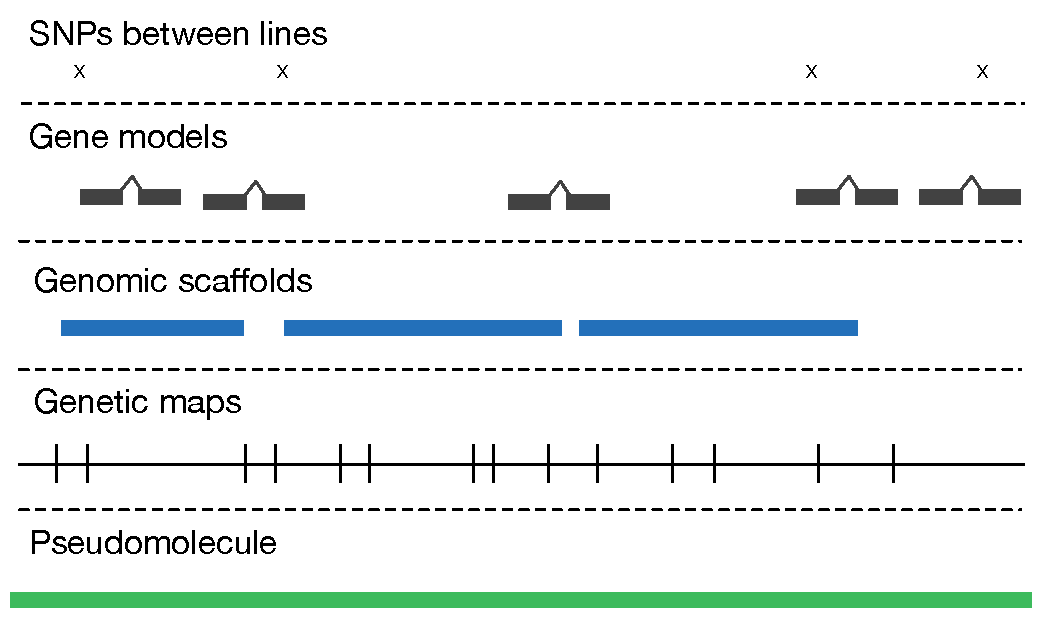
\includegraphics[width=1\textwidth]{Yr15/Figures/mapping/layersOfMapping.pdf}
  \caption[Layers of information to do \textit{In Silico} mapping.]{Layers of information to do \textit{In Silico} mapping. SNPs are called from gene models. The genes and markers from genetic maps are aligned to scaffolds. The order of the markers in a genetic map can be used to sort the scaffolds.} 
  \label{fig:yr15:layersOfMapping}
\end{figure}

Finally, the best candidate SNPs were selected to produce a genetic map which lead to a triplet of markers diagnostic for the target locus. 

The steps described in this chapter were first published in \citet{Ramirez-Gonzalez2015c} and the results of this chapter are published in \citet{Ramirez-Gonzalez2015b}.

\section{Mapping population.}

The population was developed by crossing the resistant line \gls{yr15} \citep{Wellings1998}, Figure \ref{fig:yr15.yr15Photo}, to the susceptible line \gls{avs}, Figure \ref{fig:yr15:avsPhoto}. 
\gls{yr15} is a \gls{nil} of a 6th generation \gls{bc} and the \gls{avs} background is highly susceptible to yellow rust, hence the resistance is conferred by the \gls{yr15} locus. 
$F_{2}$ seeds from three independent $F_{1}$ plants where sown and tissue was collected before fungal inoculation to avoid the effect of the disease resistance response on gene expression. 
Sampling after inoculation could have led to associations in the bulks due to expression of genes downstream of \gls{yr15} and not due to the gene itself.
Seedlings were challenged at the three leaf stage as it is known that \textit{Yr15} confers resistance in seedlings \citep{Gerechter-Amitai1989}.
The expected segregation of a $F_{2}$ population is 3:1 (resistant:susceptible), since \textit{Yr15} is a dominant gene.
From the 232 plants in the $F_{2}$ population that germinated, 187 were resistant and 45 were susceptible, which deviates slightly from the expected ratio ($\chi^{2}=0.049$).
Segregation distortion has been shown for the same \textit{Yr15} donor \citep{Randhawa2009}, however the decreased number of susceptible plants can be explained by escapes in the virulence essays (i.e. plants scored as resistant without the \textit{Yr15} locus).
For this study, we extracted DNA from individual plants in the $F_{2}$ population and we bulked RNA on 6 different bulks: 3 resistant and 3 susceptible ( Figure \ref{fig:yr15:f2}). 


\label{sub:mappingPopulation}
%\begin{SCfigure}
\begin{figure}
%\begin{wrapfigure}[17]{R!}{7cm}
    \centering
     
     \begin{subfigure}[b]{0.4\textwidth}
        \caption{}
        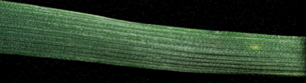
\includegraphics[width=1\textwidth]{Yr15/Figures/population/Yr15Photo.png}
        \label{fig:yr15.yr15Photo}
    \end{subfigure}
    ~
    \begin{subfigure}[b]{0.4\textwidth}
        \caption{}
        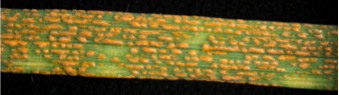
\includegraphics[width=1\textwidth]{Yr15/Figures/population/AVSPhoto.png}
        \label{fig:yr15:avsPhoto}
    \end{subfigure}

     \begin{subfigure}[b]{0.9\textwidth}
     \caption{}
        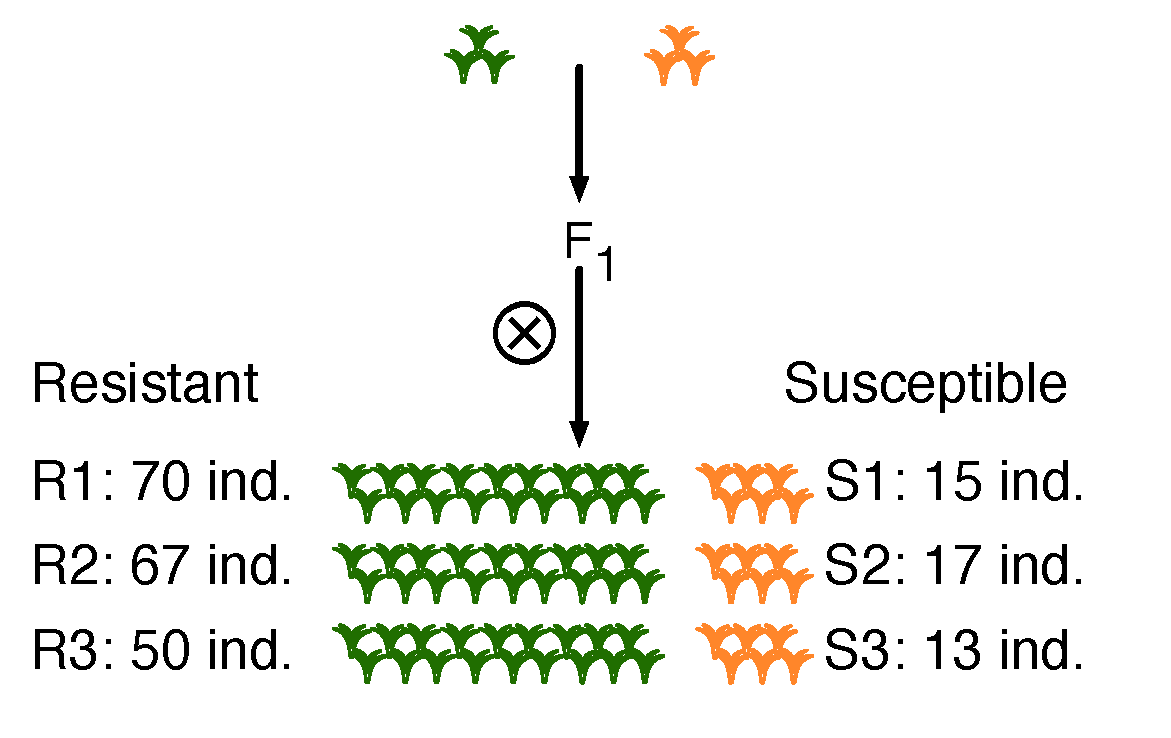
\includegraphics[width=1\textwidth]{Yr15/Figures/population/F2Population.pdf} 
    \label{fig:yr15:f2}
  \end{subfigure}

    \caption[Avocet + \textit{Yr15} $F_{2}$  mapping population.]{Avocet + \textit{Yr15} $F_{2}$  mapping population. Response of (\subref{fig:yr15.yr15Photo}) Avocet + \textit{Yr15} and (\subref{fig:yr15:avsPhoto}) Avocet when inoculated with \textit{Puccinia striiformis} f. sp.  \textit{tritici} at the three leaf stage. (\subref{fig:yr15:f2}) The phenotype of the $F_{2}$ population was used to produce 6 bulks, 3 resistant and 2 susceptible. The RNA was pooled in bulks accordingly. Adapted from \citep{Ramirez-Gonzalez2015b}}

%\end{wrapfigure}
\end{figure}
%\end{SCfigure}


\section{Sequencing and mapping.} 

RNA-Seq was used as a reduced representation method, and thus avoided sequencing the non-coding regions.
This effectively reduces the search space, which is especially important in a species with a genome as rich in repeat content as wheat.
The sequencing of the bulks and the parents was done on a single Illumina Hi-Seq2000.
The bulks were multiplexed and sequenced on a third of a lane each, as shown on Table \ref{tab:yr15:reads}. 
To ensure that quality of sequencing, \verb|fastqc-0.10| \citep{fastqc}  was run with its default parameters for each of the FASTQ files.  
The GC content was around 52\% in all the samples (Appendix \ref{App:AppendixQCGC}), which is as expected as the sample should be of coding regions, and for wheat the reported GC content in genes is around 55\%.  
The quality of the reads is fairly consistent, in general dropping after base 80 across samples (Appendix \ref{App:AppendixQCRead}). 
\label{yr15:sequencing}

\begin{table}
\centering
\caption{Arrangement and number of sequenced base pairs per sample. }
\label{tab:yr15:reads}
\begin{tabular}{rrccccc}
\toprule
Library & name & Bar code & Lane   &  Reads (\e{8} bp)\\ 
\midrule
LIB1715 & Bulk R1 & ATCACG & 1  & 0.77\\
LIB1716 & Bulk R2 & TAGCTT & 1    & 1.20\\
LIB1717 & Bulk R3 & ACTTGA & 2  & 0.96  \\ 
LIB1718 & Bulk S1 & GGCTAC & 2  & 1.64   \\ 
LIB1719 & Bulk S2 & CGTACG & 2  & 1.49  \\ 
LIB1720 & Bulk S3 & GTGGCC & 1  &1.88  \\ 
LIB1721 & AvocetS & N/A & 3     & 4.13 \\ 
LIB1722 & AvocetS + \textit{Yr15} & N/A & 4   & 3.99  \\ 
\bottomrule
\end{tabular}
\end{table}



%!TEX root = ../../Main.tex
\begin{sidewaystable}
\centering
\caption{Number of genes with a coverage over 20x, 10x and at least one read (\ensuremath{>}0x). }
\label{app:seqAlnCov}
\begin{localsize}{10}{11}

\begin{tabular}{llrrrrrr|rrrr|rr}
\toprule
          &             & \multicolumn{6}{c}{Bulks} & \multicolumn{4}{c}{Bulk  mixes} & \multicolumn{2}{c}{Progenitors}        \\
 Coverage & Reference   & R1     & R2     & R3     & S1     & S2     & S3     & R1+R2       & S1+S2  & R1+R2+R3 & S1+S2+S3 & \textit{Yr15}        & AVS     \\
 \midrule
 20x      & UCW         & 16,434 & 27,871 & 27,223 & 32,287 & 28,669 & 34,898 & 33,968      & 41,019 & 40,985   & 47,507   & 36,808      & 42,248  \\
          &             & 17\%    & 30\%    & 29\%    & 34\%    & 30\%    & 37\%    & 36\%         & 44\%    & 44\%      & 50\%      & 39\%         & 45\%     \\
          & UniGene v60 & 9,643  & 16,182 & 15,222 & 19,549 & 17,397 & 20,567 & 20,219      & 25,270 & 24,598   & 29,052   & 22,107      & 25,842  \\
          &             & 17\%    & 28\%    & 27\%    & 34\%    & 31\%    & 36\%    & 36\%         & 44\%    & 43\%      & 51\%      & 39\%         & 45\%     \\
 \midrule
 10x      & UCW         & 27,371 & 38,282 & 37,777 & 42,658 & 38,999 & 44,610 & 43,266      & 49,473 & 49,182   & 54,781   & 46,356      & 50,760  \\
          &             & 29\%    & 41\%    & 40\%    & 45\%    & 41\%    & 47\%    & 46\%         & 53\%    & 52\%      & 58\%      & 49\%         & 54\%     \\
          & UniGene v60 & 16,201 & 22,948 & 22,130 & 26,200 & 24,130 & 26,914 & 26,318      & 30,579 & 29,857   & 33,557   & 28,044      & 31,095  \\
          &             & 28\%    & 40\%    & 39\%    & 46\%    & 42\%    & 47\%    & 46\%         & 54\%    & 52\%      & 59\%      & 49\%         & 55\%     \\
 \midrule
 \ensuremath{>}0x      & UCW         & 68,302 & 72,484 & 72,957 & 74,694 & 73,290 & 75,201 & 74,397      & 77,093 & 76,715   & 78,796   & 76,275      & 77,080  \\
          &             & 73\%    & 77\%    & 77\%    & 79\%    & 78\%    & 80\%    & 79\%         & 82\%    & 81\%      & 84\%      & 81\%         & 82\%     \\
          & UniGene v60 & 40,717 & 42,489 & 42,595 & 43,625 & 43,059 & 43,748 & 43,393      & 44,655 & 44,364   & 45,392   & 43,732      & 44,596" \\
          &             & 71\%    & 75\%    & 75\%    & 77\%    & 76\%    & 77\%    & 76\%         & 78\%    & 78\%      & 80\%      & 77\%         & 78\%     \\
\bottomrule
\end{tabular}

\end{localsize}
\end{sidewaystable}


When the analysis was started, the draft genome and the corresponding annotation had not been released yet, hence gene models were used instead of a genome reference. 
All the samples were aligned to the UniGenes v60 (56,954 genes) and the gene models from UCW \citep{Krasileva2013} using \verb|BWA 0.5.9| \citep{Li2009}. 
The alignment showed that few genes were very highly expressed, however, there was still sufficient coverage of over 20x in \gls{yr15} across 22,107 and 36,808 genes, on the UniGenes and the UCW gene set, respectively. 
Both gene sets performed similarly in terms of the percentage of genes with reads and percentage of aligned reads. 
The percentage of genes with a coverage of at least $20x$ is $45\%$ and $39\%$ for \gls{avs} and \gls{yr15}, irrespective of the reference gene set chosen (Figure \ref{fig:yr15:covPerGene}).
Since each individual bulk has a lower coverage, the susceptible and resistant reads were merged \textit{in silico} as: (i) susceptible bulks 1 with 2 (S1+S2) and resistant bulks 1 with 2 (R1+R2) and (ii) all the susceptible (S1+S2+S3) and resistant bulks (R1+R2+R3). 
The merged samples increased the percentage of genes with coverage over 20x  to 44\% and 50\% in the resistant and susceptible bulks (Table \ref{app:seqAlnCov}), which is close to the coverage from the progenitors.
We treated bulk 3 slightly differently since these bulks included a few lines which were borderline with respect to their phenotype. 
Therefore exclusion of bulk 3 plants in the S1+S2 and R1+R2 bulk would provide the "cleanest" possible data, whereas inclusion in the second set of bulks would allow us to evaluate the effect of possible noise within the system. 

\begin{figure}
\centering
\begin{subfigure}{0.75\textwidth}
    \caption{}
    \centering
     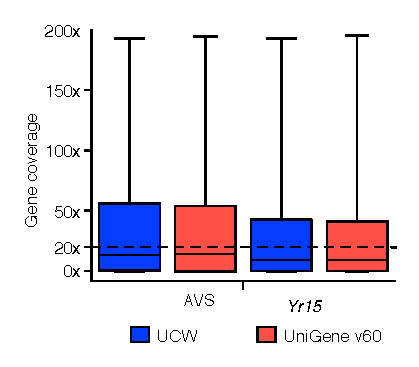
\includegraphics[height=0.25\textheight]{Yr15/Figures/CoveragePerGene.pdf} 
    \label{fig:yr15:covPerGene}
\end{subfigure}

\begin{subfigure}{0.75\textwidth}
    \caption{}
    \centering
    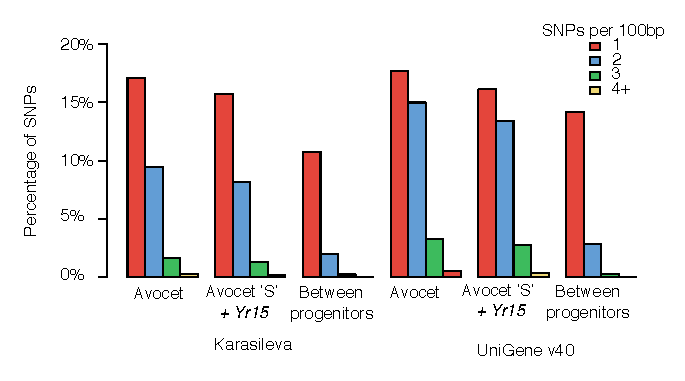
\includegraphics[height=0.25\textheight]{Yr15/Figures/PercentageOfSnps.pdf} 
    
    \label{fig:yr15:SNPper}
\end{subfigure}
\caption[Coverage and SNPs between progenitors]{Coverage and SNPs between progenitors. (\subref{fig:yr15:covPerGene}) Box plot distribution of the gene coverage of the parent reads (\gls{avs} and \gls{yr15}) across the \acrshort{ucw} (blue) and the UniGene (red) gene models. The dashed line represents the 20x minimum coverage required for SNP calling. The full line represents the average coverage across all gene models. (\subref{fig:yr15:SNPper}) Percentage of genes exhibiting SNPs across references. The number of \gls{snp}s between the parent reads and the corresponding references was calculated (per 100 bp, rounded). The ‘between-parents’ category corresponds to putative SNPs when comparing the consensus sequence between \gls{avs} and \gls{yr15} Adapted from \citet{Ramirez-Gonzalez2015b} }
\end{figure}



\section{SNP Calling}
\label{yr15:snpCalling}

The \gls{snp} calling was done on positions with a coverage of at least $20x$ on the progenitor lines against the gene reference. The \gls{avs} progenitor had roughly $3\%$ more genes with polymorphisms than \gls{yr15}, consistent with the difference in coverage, suggesting that with a higher coverage we could recover more \gls{snp}s from \gls{yr15}.
The UniGenes have a higher number of \gls{snp}s because the \gls{ucw} gene models have a higher number of monomorphic genes when compared to the UniGenes (Figure \ref{fig:yr15:SNPper}; Table \ref{app:yr15:cntSNP100bp}). 
The difference in the number of relative monomorphic SNPs between reference can be explained by the fact that in the UniGenes set many homologous might have been collapsed into a single representative sequence, whereas the \acrshort{ucw} gene set is homoeologue-specific.
Therefore, mapping to the correct homoeologue is improved in the \acrshort{ucw} gene set over the UniGenes.


%!TEX root = ../../Main.tex
\begin{table}
\caption{ Count of SNPs per 100 bp on genes with at least 20x coverage. }
\centering
\label{app:yr15:cntSNP100bp}
\begin{localsize}{10}{12}
\begin{tabular}{lrrrrrrr}
\toprule
 SNPs  & \multicolumn{3}{c}{UCW}  &  &  \multicolumn{3}{c}{UniGene v60 }                                 \\
 \cline{2-4}
 \cline{6-8}
\pbox{1cm}{per 100bp}         & AVS   & \pbox{1.5cm}{\centering AVS+ \textit{Yr15}} & \pbox{1.8cm}{\centering Between progenitors} &      & AVS         & \pbox{1.5cm}{\centering AVS+ \textit{Yr15}} & \pbox{1.8cm}{\centering Between progenitors} \\
\midrule
 0               & 67, 389       & 70,338 & 81,921             &      & 36,210       & 38,339      & 47,097               \\
                 & 71.6\% & 74.7\%      & 87.0\%               &      & 63.6\%       & 67.3\%      & 82.7\%               \\
 \midrule
 1               & 16,111 & 14,770      & 10,107               &      & 10,058       & 9,175       & 8,061                \\
                 & 17.1\% & 15.7\%      & 10.7\%               &      & 17.7\%       & 16.1\%      & 14.2\%               \\
 \midrule
 2               & 8,904  & 7,676       & 1,893                &      & 8,529	         & 7,648       & 1,621                \\
                 & 9.5\%  & 8.2\%       & 2.0\%                &      & 15.0\%       & 13.4\%      & 2.9\%                \\
 \midrule
 3               & 1,517  & 1,192       & 215                  &      & 1,870        & 1,568       & 59       \\
                 & 1.6\%  & 1.3\%       & 0.2\%                &      & 3.3\%        & 2.8\%       & 0.3\%                \\
 \midrule
 4+              & 253    & 198         & 38                   &      & 287          & 224         & 16                  \\
                 & 0.3\%  & 0.2\%       & 0.0\%                &      & 0.5\%        & 0.4\%       & 0.0\%                \\
\bottomrule
\end{tabular}
\end{localsize}
\end{table}


Both gene sets were derived from varieties different to \gls{avs} and are likely to be incomplete, hence we set a low threshold of at least 20\% of the observed nucleotides on any position to call a \gls{snp}. 
To represent cases where more than one consensus base is called we use \gls{iuapc} codes (\citet{Cornish-Bowden1985}; Section \ref{lit:ambiguity}; Figure \ref{fig:yr15:bfr}).  
To focus the analysis on informative \gls{snp}s, the common varietal SNPs and variations between homoeologues were removed by finding cases where the consensus call on both progenitors was the same. 
The \gls{snp}s that are unique to a single parental were examined in detail. 
There are 66,426 putative SNPs across 16,022 (17\%) \gls{ucw} genes and 52,262 \acrshortpl{snp} on 11,056 UniGenes (19.4\%; Figure \ref{fig:yr15:geneCount}).  

\begin{SCfigure}
    %\centering
    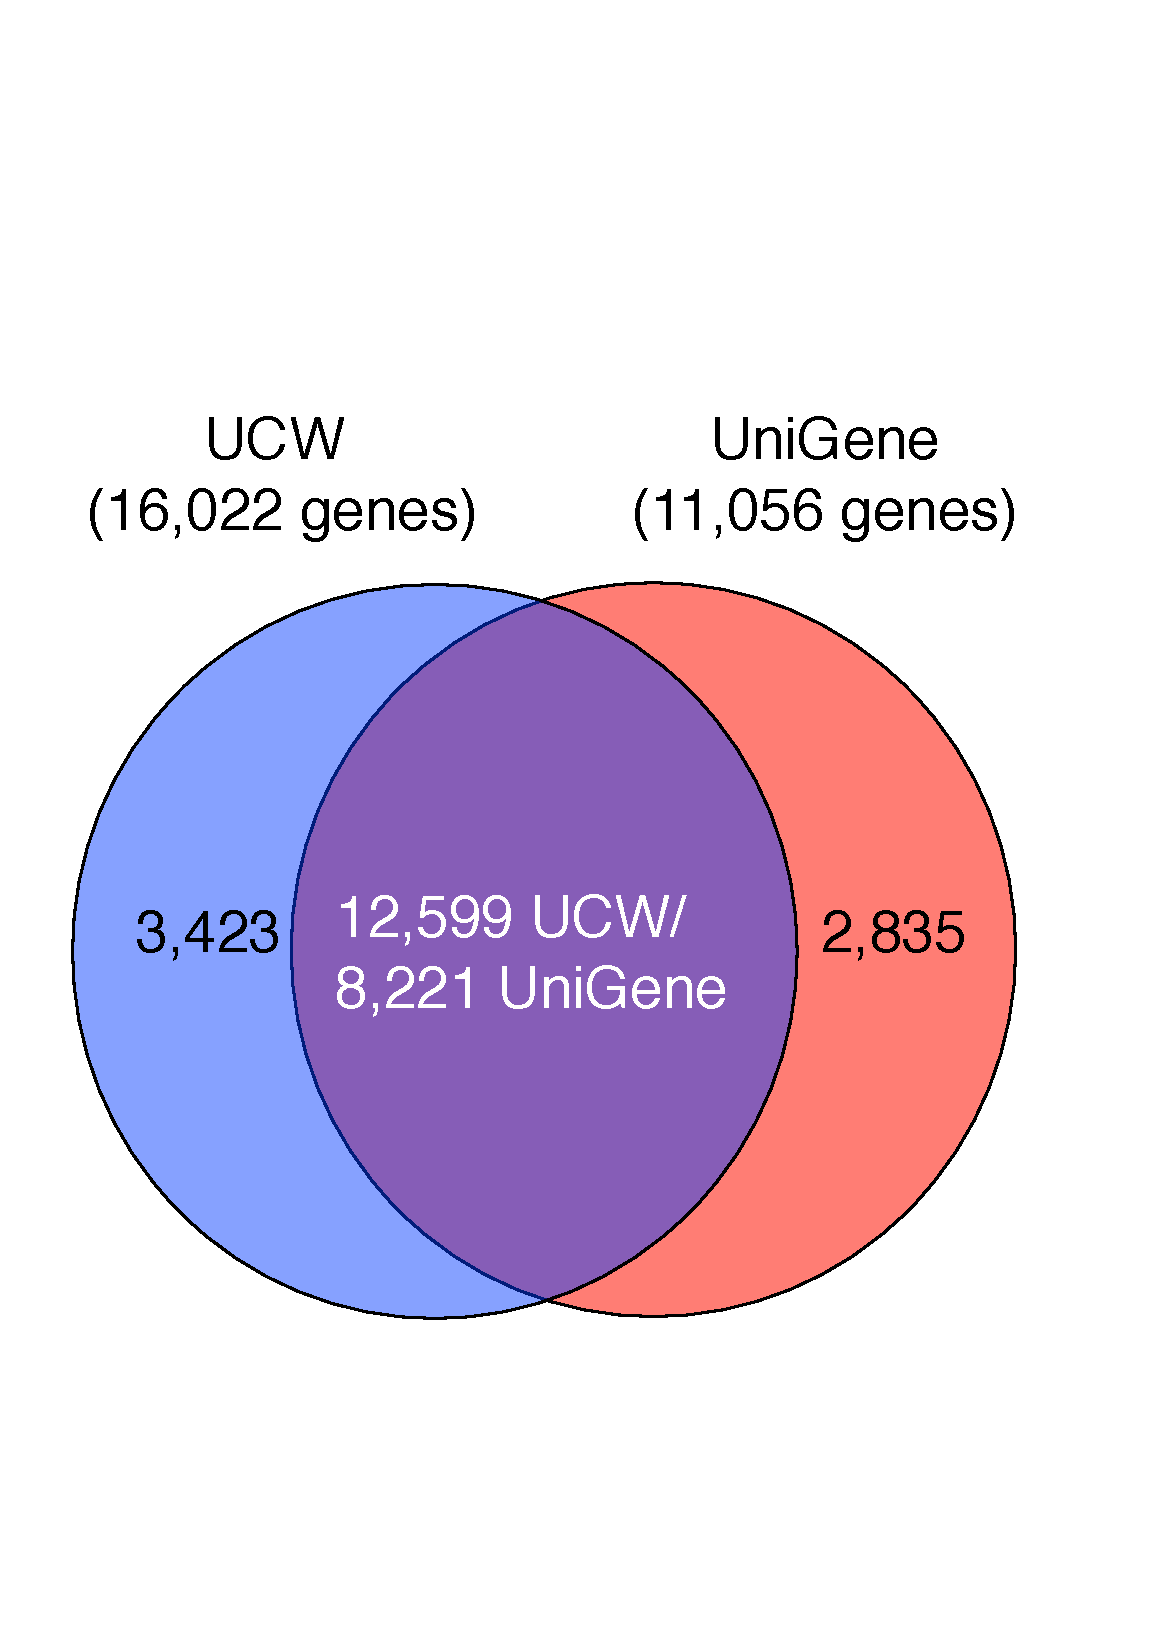
\includegraphics[width=0.4\textwidth]{Yr15/Figures/geneCounts.pdf} 
    \caption[Gene models with putative SNPs]{Gene models with putative SNPs in common between the UCW and UniGenes reference. The intersection represents the genes that are common in both sets. Adapted from \citet{Ramirez-Gonzalez2015b}}
    \label{fig:yr15:geneCount}
\end{SCfigure}

%!TEX root = ../../Main.tex
\begin{table}
\centering
\caption{ Number of genes assigned to the wheat chromosome arm CSS scaffolds \citep{Mayer2014} using the best hit from BLAT \citep{Kent2002} }
\label{tab:yr15:genesToCSS}
\begin{localsize}{10}{12}
\begin{tabular}{lrrr}
\toprule
 \pbox{2.2cm}{Wheat \\Chromosome Arm}    & UCW (94,177)    & UniGene v60 (56,954)   & Total (151,131)   \\
\midrule
 1AL                     & 3,251 (3.45\%)   & 1,404 (2.47\%)          & 4,655 (3.08\%)     \\
 1AS                     & 1,366 (1.45\%)   & 560 (0.98\%)            & 1,926 (1.27\%)     \\
 1BL                     & 2,610 (2.77\%)   & 1,280 (2.25\%)          & 3,890 (2.57\%)     \\
 1BS                     & 1,487 (1.58\%)   & 693 (1.22\%)            & 2,180 (1.44\%)     \\
 1DL                     & 997 (1.06\%)     & 1,057 (1.86\%)          & 2,054 (1.36\%)     \\
 1DS                     & 753 (0.80\%)     & 687 (1.21\%)            & 1,440 (0.95\%)     \\
 \midrule
 2AL                     & 3,491 (3.71\%)   & 1,460 (2.56\%)          & 4,951 (3.28\%)     \\
 2AS                     & 2,305 (2.45\%)   & 974 (1.71\%)            & 3,279 (2.17\%)     \\
 2BL                     & 3,658 (3.88\%)   & 1,546 (2.71\%)          & 5,204 (3.44\%)     \\
 2BS                     & 2,790 (2.96\%)   & 1,139 (2.00\%)          & 3,929 (2.60\%)     \\
 2DL                     & 1,098 (1.17\%)   & 1,069 (1.88\%)          & 2,167 (1.43\%)     \\
 2DS                     & 796 (0.85\%)     & 833 (1.46\%)            & 1,629 (1.08\%)     \\
 \midrule
 3AL                     & 2,135 (2.27\%)   & 978 (1.72\%)            & 3,113 (2.06\%)     \\
 3AS                     & 1,543 (1.64\%)   & 718 (1.26\%)            & 2,261 (1.50\%)     \\
 3B                      & 6,559 (6.96\%)   & 2,839 (4.98\%)          & 9,398 (6.22\%)     \\
 3DL                     & 915 (0.97\%)     & 938 (1.65\%)            & 1,853 (1.23\%)     \\
 3DS                     & 412 (0.44\%)     & 450 (0.79\%)            & 862 (0.57\%)       \\
 \midrule
 4AL                     & 3,393 (3.60\%)   & 1,335 (2.34\%)          & 4,728 (3.13\%)     \\
 4AS                     & 2,011 (2.14\%)   & 817 (1.43\%)            & 2,828 (1.87\%)     \\
 4BL                     & 2,119 (2.25\%)   & 898 (1.58\%)            & 3,017 (2.00\%)     \\
 4BS                     & 1,946 (2.07\%)   & 892 (1.57\%)            & 2,838 (1.88\%)     \\
 4DL                     & 1,069 (1.14\%)   & 945 (1.66\%)            & 2,014 (1.33\%)     \\
 4DS                     & 800 (0.85\%)     & 699 (1.23\%)            & 1,499 (0.99\%)     \\
 \midrule
 5AL                     & 2,640 (2.80\%)   & 1,132 (1.99\%)          & 3,772 (2.50\%)     \\
 5AS                     & 963 (1.02\%)     & 407 (0.71\%)            & 1,370 (0.91\%)     \\
 5BL                     & 5,324 (5.65\%)   & 1,943 (3.41\%)          & 7,267 (4.81\%)     \\
 5BS                     & 1,360 (1.44\%)   & 591 (1.04\%)            & 1,951 (1.29\%)     \\
 5DL                     & 2,067 (2.19\%)   & 1,688 (2.96\%)          & 3,755 (2.48\%)     \\
 5DS                     & 620 (0.66\%)     & 614 (1.08\%)            & 1,234 (0.82\%)     \\
 \midrule
 6AL                     & 2,397 (2.55\%)   & 896 (1.57\%)            & 3,293 (2.18\%)     \\
 6AS                     & 2,285 (2.43\%)   & 936 (1.64\%)            & 3,221 (2.13\%)     \\
 6BL                     & 1,564 (1.66\%)   & 820 (1.44\%)            & 2,384 (1.58\%)     \\
 6BS                     & 1,308 (1.39\%)   & 731 (1.28\%)            & 2,039 (1.35\%)     \\
 6DL                     & 1,399 (1.49\%)   & 1,050 (1.84\%)          & 2,449 (1.62\%)     \\
 6DS                     & 870 (0.92\%)     & 680 (1.19\%)            & 1,550 (1.03\%)     \\
 \midrule
 7AL                     & 1,918 (2.04\%)   & 849 (1.49\%)            & 2,767 (1.83\%)     \\
 7AS                     & 1,717 (1.82\%)   & 764 (1.34\%)            & 2,481 (1.64\%)     \\
 7BL                     & 1,592 (1.69\%)   & 776 (1.36\%)            & 2,368 (1.57\%)     \\
 7BS                     & 1,239 (1.32\%)   & 713 (1.25\%)            & 1,952 (1.29\%)     \\
 7DL                     & 2,040 (2.17\%)   & 1,301 (2.28\%)          & 3,341 (2.21\%)     \\
 7DS                     & 1,224 (1.30\%)   & 1,016 (1.78\%)          & 2,240 (1.48\%)     \\
 \midrule
 Assigned                & 80,031 (84.98\%) & 41,118 (72.20\%)        & 121,149 (80.16\%)  \\
\bottomrule
\end{tabular}
\end{localsize}
\end{table}

The high number of genes with \gls{snp}s was unexpected as a \gls{bc}6 \gls{nil} used for a $F_2$ mapping population expects to have less than $1\%$ of the genetic background segregating. 
Both sets of gene models were aligned with BLAT \citep{Kent2002} to the \gls{css} assembly \citep{Mayer2014}; the alignment resulted on 80,031 (85.0\%) \acrshort{ucw} gene models and 41,118 (72.2\%) UniGenes assigned to a chromosome arm (Table \ref{tab:yr15:genesToCSS}). 
The SNPs found in the mapped genes are evenly distributed across all the chromosomes (see Section \ref{sub:yr15:inSilico}), suggesting that the \gls{avs} (\gls{jic}, UK) used as parent in the $F_{2}$ is different to the \gls{avs} used for the \acrshort{yr15} \acrshort{nil} development (University of Sydney, Australia).  

To confirm that the \gls{avs} seed stocks from \gls{jic} are distinct to the stocks in Sydney, DNA from both stocks was procured and compared with the iSelect 90k wheat SNP chip. 
Between two independent \gls{avs} seeds from \gls{jic} only 58 out of 71,972 (0.08\%) valid assays were polymorphic. 
Nonetheless, there are over 5,000 ($>7.5\%$) assays with polymorphisms between  \gls{jic}-\gls{avs} and \gls{avs} from Sydney. 
The difference was not expected originally, but considering that the \gls{avs} seeds are coming from different stocks and the fact that in both countries commercial varieties with the same name had been released, it is not surprising. 


\section{Bulk Frequency Ratios}
\label{sec:yr15:bfr}

%!TEX root = ../../Main.tex
\begin{table}
\caption{Total number of SNPs scored in parents, individual bulks and in silico merged bulks. }
\centering
\label{app:yr15:scoredSNPs}
\begin{localsize}{10}{12}
\begin{tabular}{lrrrrrr}
\toprule
 Gene set    & $\frac{R1}{S1}$  & $\frac{R2}{S2}$   & $\frac{R3}{S3}$   & $\frac{R1+R2}{S1+S2}$    & $\frac{R1+R2+R3}{S1+S2+S3}$   & \pbox{1.8cm}{\centering SNPs in  parents}   \\
\midrule
 UCW         & 16,269  & 29,703  & 31,891  & 44,224         & 64,522               & 66,426            \\
             & 24.49\%  & 44.72\%  & 48.01\%  & 66.58\%         & 97.13\%               &                   \\
\midrule
 UniGene v60 & 15,261  & 25,143  & 24,548  & 35,698         & 49,738               & 52,262            \\
             & 29.20\%  & 48.11\%  & 46.97\%  & 68.31\%         & 95.17\%               &                   \\
\bottomrule
\end{tabular}
\end{localsize}
\end{table}

The objective was to find the SNPs enriched (or depleted) in each bulk and hence linked to the phenotype.  \Glspl{snp} originating from \gls{yr15} would be expected to be linked to resistance whereas those from \acrshort{avs} to susceptibility in the segregating population. 
Across individual bulks, it was possible to score between 15,261 (24.5\%) and 31,891(48.0\%) \glspl{snp}s across both reference sets.
On the \textit{in silico} mixes, over $95\%$ of SNPs where scored (Table \ref{app:yr15:scoredSNPs}), suggesting that the coverage of individual bulks is not enough to score all the SNPs.
The scoring was done with the \acrlong{bfr} (\citealt{Trick2012};Figure \ref{fig:yr15:bfr}; Section \ref{yr15:sub:bfr}), which has a value that increases as the \acrshort{yr15} allele is observed more times relatively to the \acrshort{avs} allele.

%!TEX root = ../../Main.tex
\begin{sidewaystable}
\caption{ SNPs in chromosome group 1S vs total number of SNPs with a minimum BFR from 0 to 10. AVS: SNPs coming from \acrlong{avs}. \textit{Yr15}: SNPs comming from \acrlong{yr15}. }
\centering
\label{app:yr15:bfrThresholds}
\begin{localsize}{6}{7}

\begin{tabular}{llp{1cm}p{1cm}p{1cm}p{1cm}p{1cm}p{1cm}p{1cm}p{1cm}p{1cm}p{1cm}}
\toprule
 Min  BFR   & Gene Set    & R1/S1 \textit{Yr15}        & R1/S1 AVS         & R2/S2 \textit{Yr15}         & R2/S2 AVS          & R3/S3 \textit{Yr15}         & R3/S3 AVS          & S1+2/ R1+2 \textit{Yr15}    & S1+2/ R1+2 AVS     & S1+S2+S3/ R1+R2+R3 \textit{Yr15}   & S1+S2+S3/ R1+R2+R3 AVS   \\
\midrule
 0          & UCW         & 308/8,049 (3.83\%) & 305/8,220 (3.71\%) & 505/14,121 (3.58\%) & 556/15,582 (3.57\%) & 532/14,875 (3.58\%) & 623/17,016 (3.66\%) & 670/18,760 (3.57\%) & 885/25,464 (3.48\%) & 860/24,026 (3.58\%)        & 1,505/40,496 (3.72\%)     \\
            & UniGene v60 & 307/7,823 (3.92\%) & 299/7,438 (4.02\%) & 428/12,409 (3.45\%) & 421/12,734 (3.31\%) & 427/12,050 (3.54\%) & 415/12,498 (3.32\%) & 536/15,672 (3.42\%) & 595/20,026 (2.97\%) & 712/19,358 (3.68\%)        & 901/30,380 (2.97\%)       \\
 \midrule
 1          & UCW         & 214/4,415 (4.85\%) & 194/4,108 (4.72\%) & 325/7,603 (4.27\%)  & 314/7,374 (4.26\%)  & 365/7,920 (4.61\%)  & 415/8,850 (4.69\%)  & 426/10,122 (4.21\%) & 494/12,185 (4.05\%) & 539/13,037 (4.13\%)        & 842/19,466 (4.33\%)       \\
            & UniGene v60 & 207/4,474 (4.63\%) & 194/3,630 (5.34\%) & 269/6,649 (4.05\%)  & 269/6,193 (4.34\%)  & 279/6,511 (4.29\%)  & 272/6,436 (4.23\%)  & 329/8,704 (3.78\%)  & 369/9,343 (3.95\%)  & 446/10,860 (4.11\%)        & 541/14,226 (3.80\%)       \\
 \midrule
 2          & UCW         & 92/651 (14.13\%)   & 75/671 (11.18\%)   & 142/1,372 (10.35\%) & 111/1,101 (10.08\%) & 147/1,162 (12.65\%) & 149/1,411 (10.56\%) & 167/1,324 (12.61\%) & 163/1,478 (11.03\%) & 194/1,370 (14.16\%)        & 207/1,765 (11.73\%)       \\
            & UniGene v60 & 77/568 (13.56\%)   & 58/527 (11.01\%)   & 101/1,017 (9.93\%)  & 81/720 (11.25\%)    & 105/775 (13.55\%)   & 84/867 (9.69\%)     & 122/991 (12.31\%)   & 116/973 (11.92\%)   & 145/1,030 (14.08\%)        & 132/1,210 (10.91\%)       \\
 \midrule
 3          & UCW         & 78/299 (26.09\%)   & 45/295 (15.25\%)   & 118/646 (18.27\%)   & 70/409 (17.11\%)    & 123/577 (21.32\%)   & 85/494 (17.21\%)    & 145/673 (21.55\%)   & 98/563 (17.41\%)    & 168/768 (21.88\%)          & 122/665 (18.35\%)         \\
            & UniGene v60 & 65/254 (25.59\%)   & 26/186 (13.98\%)   & 87/499 (17.43\%)    & 54/294 (18.37\%)    & 93/379 (24.54\%)    & 48/315 (15.24\%)    & 107/525 (20.38\%)   & 66/379 (17.41\%)    & 133/617 (21.56\%)          & 78/489 (15.95\%)          \\
 \midrule
 4          & UCW         & 75/232 (32.33\%)   & 28/160 (17.50\%)   & 109/484 (22.52\%)   & 44/217 (20.28\%)    & 105/416 (25.24\%)   & 44/246 (17.89\%)    & 134/539 (24.86\%)   & 53/277 (19.13\%)    & 149/640 (23.28\%)          & 64/323 (19.81\%)          \\
            & UniGene v60 & 63/192 (32.81\%)   & 17/104 (16.35\%)   & 83/390 (21.28\%)    & 29/155 (18.71\%)    & 82/288 (28.47\%)    & 29/173 (16.76\%)    & 104/431 (24.13\%)   & 40/214 (18.69\%)    & 127/519 (24.47\%)          & 29/266 (10.90\%)          \\
 \midrule
 5          & UCW         & 69/202 (34.16\%)   & 19/108 (17.59\%)   & 95/416 (22.84\%)    & 33/138 (23.91\%)    & 96/354 (27.12\%)    & 23/143 (16.08\%)    & 127/477 (26.62\%)   & 28/175 (16.00\%)    & 140/580 (24.14\%)          & 42/222 (18.92\%)          \\
            & UniGene v60 & 58/163 (35.58\%)   & 11/70 (15.71\%)    & 76/337 (22.55\%)    & 14/102 (13.73\%)    & 70/228 (30.70\%)    & 20/112 (17.86\%)    & 100/389 (25.71\%)   & 23/146 (15.75\%)    & 118/469 (25.16\%)          & 21/178 (11.80\%)          \\
 \midrule
 6          & UCW         & 65/179 (36.31\%)   & 12/85 (14.12\%)    & 86/380 (22.63\%)    & 22/98 (22.45\%)     & 87/299 (29.10\%)    & 11/94 (11.70\%)     & 122/429 (28.44\%)   & 21/130 (16.15\%)    & 126/514 (24.51\%)          & 29/165 (17.58\%)          \\
            & UniGene v60 & 57/151 (37.75\%)   & 7/48 (14.58\%)     & 73/300 (24.33\%)    & 6/71     (8.45\%)   & 65/191 (34.03\%)    & 13/84 (15.48\%)     & 98/358 (27.37\%)    & 20/122 (16.39\%)    & 115/439 (26.20\%)          & 16/143 (11.19\%)          \\
 \midrule
 7          & UCW         & 58/161 (36.02\%)   & 11/73 (15.07\%)    & 77/340 (22.65\%)    & 13/74 (17.57\%)     & 73/248 (29.44\%)    & 7/69 (10.14\%)      & 116/393 (29.52\%)   & 20/111 (18.02\%)    & 114/468 (24.36\%)          & 22/143 (15.38\%)          \\
            & UniGene v60 & 56/132 (42.42\%)   & 4/37 (10.81\%)     & 68/273 (24.91\%)    & 5/58    (8.62\%)    & 60/171 (35.09\%)    & 9/64 (14.06\%)      & 94/334 (28.14\%)    & 18/103 (17.48\%)    & 113/412 (27.43\%)          & 16/124 (12.90\%)          \\
 \midrule
 8          & UCW         & 58/149 (38.93\%)   & 10/62 (16.13\%)    & 68/310 (21.94\%)    & 12/59 (20.34\%)     & 66/214 (30.84\%)    & 6/56 (10.71\%)      & 104/359 (28.97\%)   & 17/102 (16.67\%)    & 108/429 (25.17\%)          & 16/119 (13.45\%)          \\
            & UniGene v60 & 55/126 (43.65\%)   & 3/33    (9.09\%)   & 64/255 (25.10\%)    & 5/50 (10.00\%)      & 55/150 (36.67\%)    & 9/55 (16.36\%)      & 91/313 (29.07\%)    & 14/89 (15.73\%)     & 105/376 (27.93\%)          & 15/108 (13.89\%)          \\
 \midrule
 9          & UCW         & 54/135 (40.00\%)   & 8/53 (15.09\%)     & 63/289 (21.80\%)    & 8/51 (15.69\%)      & 61/182 (33.52\%)    & 5/49 (10.20\%)      & 100/331 (30.21\%)   & 15/91 (16.48\%)     & 100/387 (25.84\%)          & 13/106 (12.26\%)          \\
            & UniGene v60 & 53/117 (45.30\%)   & 1/30    (3.33\%)   & 62/244 (25.41\%)    & 5/46 (10.87\%)      & 50/136 (36.76\%)    & 9/48 (18.75\%)      & 88/291 (30.24\%)    & 13/83 (15.66\%)     & 97/345 (28.12\%)           & 12/99 (12.12\%)           \\
 \midrule
 10         & UCW         & 52/126 (41.27\%)   & 8/50 (16.00\%)     & 62/279 (22.22\%)    & 8/50 (16.00\%)      & 56/165 (33.94\%)    & 4/45    (8.89\%)    & 96/309 (31.07\%)    & 14/82 (17.07\%)     & 91/355 (25.63\%)           & 13/100 (13.00\%)          \\
            & UniGene v60 & 50/105 (47.62\%)   & 1/28    (3.57\%)   & 60/226 (26.55\%)    & 5/39 (12.82\%)      & 43/119 (36.13\%)    & 7/45 (15.56\%)      & 85/272 (31.25\%)    & 13/82 (15.85\%)     & 92/318 (28.93\%)           & 12/97 (12.37\%)           \\
\bottomrule
\end{tabular}
\end{localsize}
\end{sidewaystable}


When increasing the minimum \acrshort{bfr} threshold, enrichment of SNPs was observed in the short arm of the group 1 chromosomes (1S). 
Without taking into account the \acrshort{bfr}, $~3.6\%$ of the SNPs are located in the 1S group, similar to the number of SNPs located in other groups \ref{tab:yr15:genesToCSS}. 
However, when increasing the threshold  (between $BFR > 5 $ and $BFR > 7$) the relative number of SNPs in group 1S increases. 
After $BFR>7$ the gains in relative enrichment only improves marginally, but the number of called SNPs is reduced (Table \ref{app:yr15:bfrThresholds}; Figure \ref{fig:yr15:bfrChange}).
For that reason, SNPs with a $BFR>6$ were selected for further validation. 
The method described by \citet{Trick2012} was extended to include cases where there is a complete lack of coverage in one of the samples ($BFR=\infty$), which is an ideal case where the linkage between the SNP and the phenotype is perfect. 
A total of 1,582 SNPs across 1,173 genes had a $BFR>6$.



\begin{sidewaysfigure}
\centering
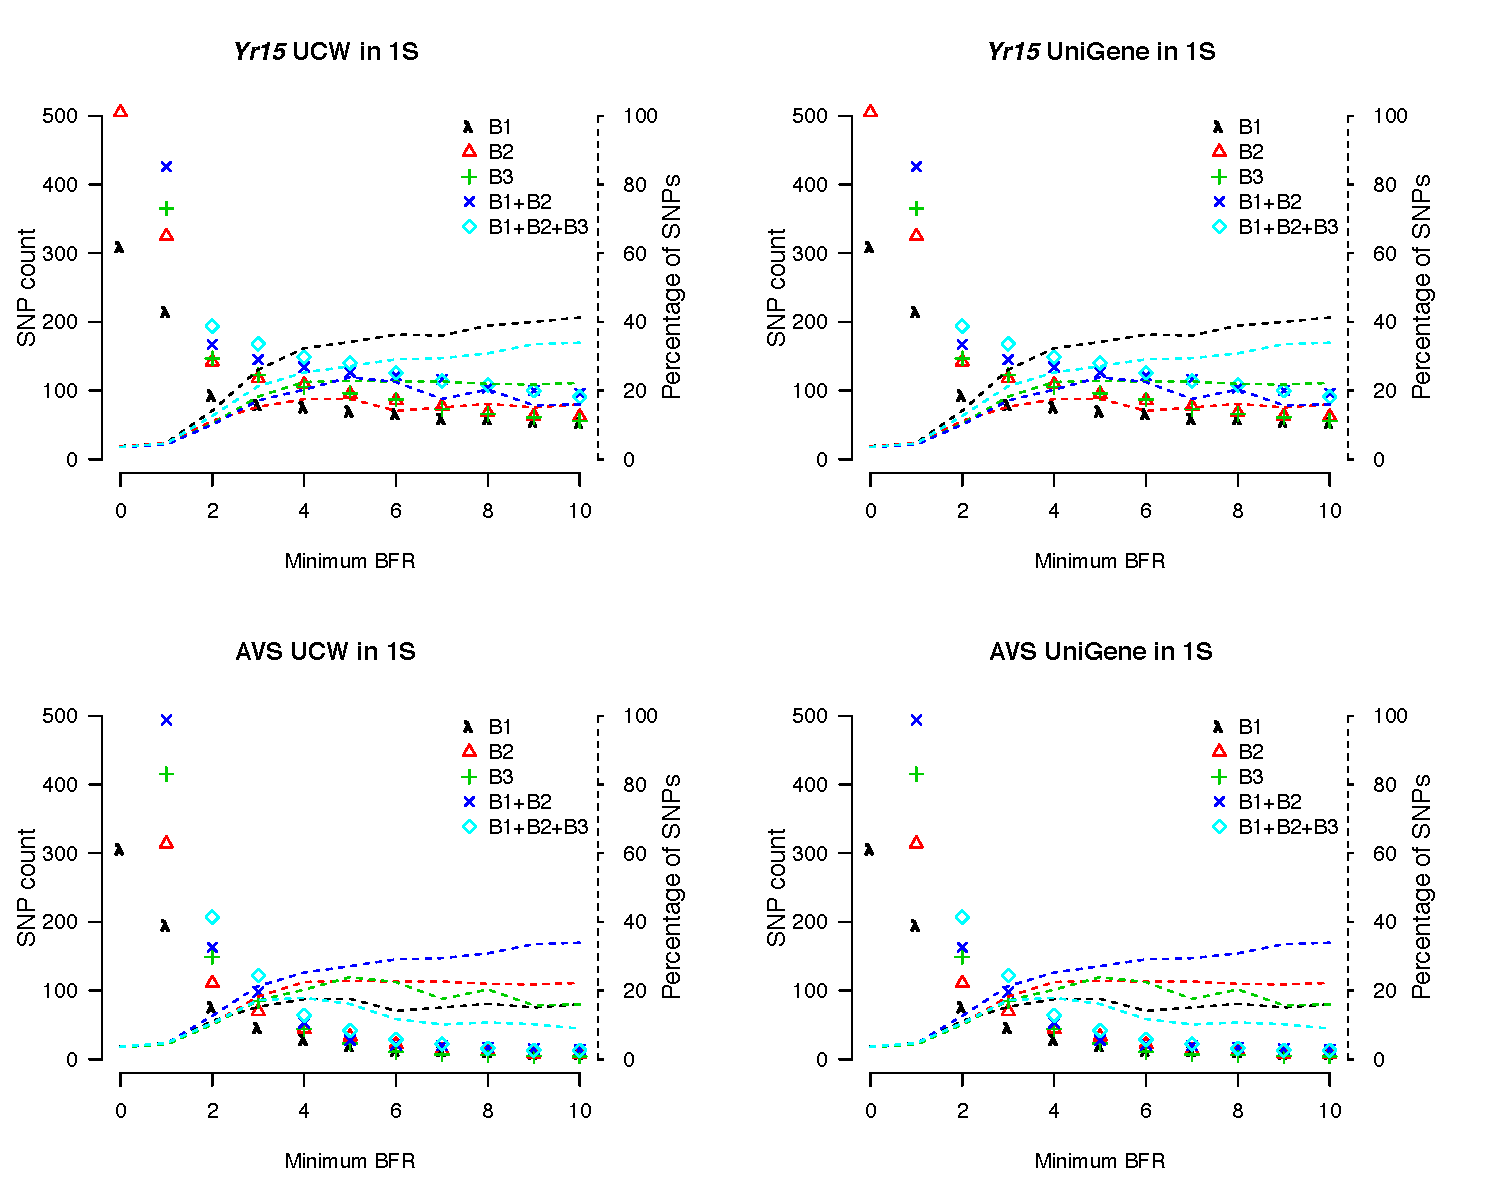
\includegraphics[width=0.8\textwidth]{Yr15/Figures/bfrChanges.pdf}
\caption[Effect of BFR threshold on the number of SNPs]{Effect of BFR threshold on the number of SNPs across the short arm of chromosome group 1. Count of SNPs with across different BFR threshold, in the short arm of chromosome group 1.  Top row: SNPs from AVS+\textit{Yr15}; Bottom row: AVS; Left: UCW gene models: Right: UniGene v60. On dotted lines, the percentage of SNPs that map to the group 1S. The symbols represent the count of SNPs. The count of SNPs from AVS decreases faster than the count of SNPs from AVS+\textit{Yr15} across the bulks.  Figure previously published in \citet{Ramirez-Gonzalez2015b}. }
\label{fig:yr15:bfrChange}
\end{sidewaysfigure}

\section{\textit{In silico} mapping}
\label{sub:yr15:inSilico}
From the mapped SNPs with a $BFR>6$, 872 of 1,582 ($\sim60\%$) were assigned to the chromosomes in group 1 of hexaploid wheat, being the only group with more than $4\%$ of the SNPs assigned to it (Table \ref{app:yr15:bfr6Mapping}). 
From group 1, the B genome contained the higher proportion of SNPs mapped ($54\%$), having 255 ($54\%$) and 214 ($46\%$) assigned to the long and short arms respectively (Figure \ref{fig:yr15:snpsBFR6Group1}).  
These results are expected since previous studies have located \acrshort{yr15} near the centromere in the short arm of chromosome 1B and the \acrshort{yr15} introgression contains regions from the long and short arm from \textit{T. dicoccoides} \citep{Murphy2009,Peng2000,Grama1997}. 

\begin{SCfigure}
  \centering
    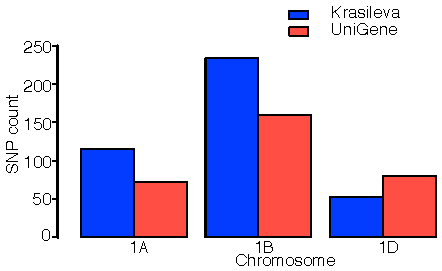
\includegraphics[width=0.5\textwidth]{Yr15/Figures/mapping/snpsBFR6Group1.pdf}
  \caption[Location of SNPs with BFR\textgreater6.]{Location of SNPs with $BFR>6$ according to the best alignment of the UniGene (red) and UCW (blue) gene models to the flow-sorted group 1 chromosomes from the \gls{css} \citep{Mayer2014}. Figure adapted from \citet{Ramirez-Gonzalez2015b}.} 
  \label{fig:yr15:snpsBFR6Group1}
\end{SCfigure}

%!TEX root = ../../Main.tex
\begin{sidewaystable}
\caption{ SNP and genes with BFR > 6 mapping to each of the chromosomes from the CSS assemblies. The chromosome assignment on the "Genetically mapped" column correspond to the map published in \citet{Wang2014}). }
\centering
\label{app:yr15:bfr6Mapping}
\begin{localsize}{6}{9}

\begin{tabular}{rrrrrrrrrrrrrrrrrrrr}
\toprule
Reference & \multicolumn{9}{c}{CSS assemblies}        &    & \multicolumn{9}{c}{Genetically mapped}   \\
 \cline{2-10}
 \cline{12-20}
Chromosome & \multicolumn{4}{c}{UCW gene models} &    & \multicolumn{4}{c}{UniGene v60}&    & \multicolumn{4}{c}{UCW gene models} &    & \multicolumn{4}{c}{UniGene v60}        \\

 \cline{2-5}
 \cline{7-10}
  \cline{12-15}
 \cline{17-20}
 %\midrule
  arm & 
 \multicolumn{2}{c}{SNPs } & 
 \multicolumn{2}{c}{Genes } &  &
 \multicolumn{2}{c}{SNPs } & 
 \multicolumn{2}{c}{Genes } &     &  
 \multicolumn{2}{c}{SNPs } & 
 \multicolumn{2}{c}{Genes } & &
 \multicolumn{2}{c}{SNPs } & 
 \multicolumn{2}{c}{Genes }      
 \\
 \midrule
 1AL            & 113                   & 13.15\% & 79    & 12.29\% &    & 78          & 10.79\% & 50    & 9.43\%  &    & 14                     & 1.63\%  & 8     & 1.24\%  &    & 7           & 0.97\%  & 4     & 0.75\%  \\
 1AS            & 26                    & 3.03\%  & 21    & 3.27\%  &    & 20          & 2.77\%  & 17    & 3.21\%  &    & 42                     & 4.89\%  & 32    & 4.98\%  &    & 38          & 5.26\%  & 28    & 5.28\%  \\
 1BL            & 157                   & 18.28\% & 110   & 17.11\% &    & 98          & 13.55\% & 64    & 12.08\% &    & 60                     & 6.98\%  & 35    & 5.44\%  &    & 36          & 4.98\%  & 23    & 4.34\%  \\
 1BS            & 120                   & 13.97\% & 74    & 11.51\% &    & 94          & 13.00\% & 44    & 8.30\%  &    & 127                    & 14.78\% & 80    & 12.44\% &    & 102         & 14.11\% & 46    & 8.68\%  \\
 1DL            & 30                    & 3.49\%  & 21    & 3.27\%  &    & 58          & 8.02\%  & 47    & 8.87\%  &    & 2                      & 0.23\%  & 2     & 0.31\%  &    & 4           & 0.55\%  & 4     & 0.75\%  \\
 1DS            & 40                    & 4.66\%  & 25    & 3.89\%  &    & 38          & 5.26\%  & 24    & 4.53\%  &    & 12                     & 1.40\%  & 6     & 0.93\%  &    & 8           & 1.11\%  & 5     & 0.94\%  \\
  \midrule
 2AL            & 22                    & 2.56\%  & 20    & 3.11\%  &    & 14          & 1.94\%  & 12    & 2.26\%  &    & 9                      & 1.05\%  & 8     & 1.24\%  &    & 7           & 0.97\%  & 5     & 0.94\%  \\
 2AS            & 11                    & 1.28\%  & 11    & 1.71\%  &    & 10          & 1.38\%  & 7     & 1.32\%  &    & 9                      & 1.05\%  & 9     & 1.40\%  &    & 2           & 0.28\%  & 2     & 0.38\%  \\
 2BL            & 17                    & 1.98\%  & 15    & 2.33\%  &    & 18          & 2.49\%  & 17    & 3.21\%  &    & 7                      & 0.81\%  & 5     & 0.78\%  &    & 4           & 0.55\%  & 4     & 0.75\%  \\
 2BS            & 11                    & 1.28\%  & 10    & 1.56\%  &    & 12          & 1.66\%  & 7     & 1.32\%  &    & 13                     & 1.51\%  & 12    & 1.87\%  &    & 7           & 0.97\%  & 7     & 1.32\%  \\
 2DL            & 2                     & 0.23\%  & 2     & 0.31\%  &    & 15          & 2.07\%  & 10    & 1.89\%  &    & 1                      & 0.12\%  & 1     & 0.16\%  &    & 3           & 0.41\%  & 2     & 0.38\%  \\
 2DS            & 0                     & 0.00\%  & 0     & 0.00\%  &    & 5           & 0.69\%  & 3     & 0.57\%  &    & 0                      & 0.00\%  & 0     & 0.00\%  &    & 0           & 0.00\%  & 0     & 0.00\%  \\
  \midrule
  3AL            & 7                     & 0.81\%  & 7     & 1.09\%  &    & 2           & 0.28\%  & 2     & 0.38\%  &    & 2                      & 0.23\%  & 2     & 0.31\%  &    & 1           & 0.14\%  & 1     & 0.19\%  \\
 3AS            & 1                     & 0.12\%  & 1     & 0.16\%  &    & 4           & 0.55\%  & 4     & 0.75\%  &    & 0                      & 0.00\%  & 0     & 0.00\%  &    & 0           & 0.00\%  & 0     & 0.00\%  \\
 3B             & 31                    & 3.61\%  & 26    & 4.04\%  &    & 28          & 3.87\%  & 24    & 4.53\%  &    & 0                      & 0.00\%  & 0     & 0.00\%  &    & 0           & 0.00\%  & 0     & 0.00\%  \\
 3BL            & 0                     & 0.00\%  & 0     & 0.00\%  &    & 0           & 0.00\%  & 0     & 0.00\%  &    & 9                      & 1.05\%  & 7     & 1.09\%  &    & 4           & 0.55\%  & 4     & 0.75\%  \\
 3BS            & 0                     & 0.00\%  & 0     & 0.00\%  &    & 0           & 0.00\%  & 0     & 0.00\%  &    & 2                      & 0.23\%  & 2     & 0.31\%  &    & 5           & 0.69\%  & 5     & 0.94\%  \\
 3DL            & 7                     & 0.81\%  & 6     & 0.93\%  &    & 2           & 0.28\%  & 2     & 0.38\%  &    & 1                      & 0.12\%  & 1     & 0.16\%  &    & 0           & 0.00\%  & 0     & 0.00\%  \\
 3DS            & 1                     & 0.12\%  & 1     & 0.16\%  &    & 2           & 0.28\%  & 2     & 0.38\%  &    & 0                      & 0.00\%  & 0     & 0.00\%  &    & 0           & 0.00\%  & 0     & 0.00\%  \\
  \midrule
  4AL            & 18                    & 2.10\%  & 15    & 2.33\%  &    & 6           & 0.83\%  & 6     & 1.13\%  &    & 14                     & 1.63\%  & 11    & 1.71\%  &    & 5           & 0.69\%  & 4     & 0.75\%  \\
 4AS            & 5                     & 0.58\%  & 5     & 0.78\%  &    & 6           & 0.83\%  & 5     & 0.94\%  &    & 0                      & 0.00\%  & 0     & 0.00\%  &    & 0           & 0.00\%  & 0     & 0.00\%  \\
 4BL            & 11                    & 1.28\%  & 10    & 1.56\%  &    & 6           & 0.83\%  & 6     & 1.13\%  &    & 3                      & 0.35\%  & 3     & 0.47\%  &    & 4           & 0.55\%  & 4     & 0.75\%  \\
 4BS            & 6                     & 0.70\%  & 5     & 0.78\%  &    & 13          & 1.80\%  & 10    & 1.89\%  &    & 4                      & 0.47\%  & 3     & 0.47\%  &    & 4           & 0.55\%  & 3     & 0.57\%  \\
 4DL            & 4                     & 0.47\%  & 4     & 0.62\%  &    & 5           & 0.69\%  & 5     & 0.94\%  &    & 0                      & 0.00\%  & 0     & 0.00\%  &    & 1           & 0.14\%  & 1     & 0.19\%  \\
 4DS            & 2                     & 0.23\%  & 2     & 0.31\%  &    & 5           & 0.69\%  & 4     & 0.75\%  &    & 0                      & 0.00\%  & 0     & 0.00\%  &    & 1           & 0.14\%  & 1     & 0.19\%  \\
  \midrule
  5AL            & 7                     & 0.81\%  & 5     & 0.78\%  &    & 3           & 0.41\%  & 3     & 0.57\%  &    & 3                      & 0.35\%  & 2     & 0.31\%  &    & 1           & 0.14\%  & 1     & 0.19\%  \\
 5AS            & 1                     & 0.12\%  & 1     & 0.16\%  &    & 2           & 0.28\%  & 2     & 0.38\%  &    & 1                      & 0.12\%  & 1     & 0.16\%  &    & 1           & 0.14\%  & 1     & 0.19\%  \\
 5BL            & 31                    & 3.61\%  & 28    & 4.35\%  &    & 14          & 1.94\%  & 14    & 2.64\%  &    & 12                     & 1.40\%  & 12    & 1.87\%  &    & 6           & 0.83\%  & 6     & 1.13\%  \\
 5BS            & 7                     & 0.81\%  & 5     & 0.78\%  &    & 6           & 0.83\%  & 5     & 0.94\%  &    & 2                      & 0.23\%  & 2     & 0.31\%  &    & 1           & 0.14\%  & 1     & 0.19\%  \\
 5DL            & 8                     & 0.93\%  & 7     & 1.09\%  &    & 15          & 2.07\%  & 14    & 2.64\%  &    & 2                      & 0.23\%  & 2     & 0.31\%  &    & 6           & 0.83\%  & 6     & 1.13\%  \\
 5DS            & 4                     & 0.47\%  & 3     & 0.47\%  &    & 6           & 0.83\%  & 5     & 0.94\%  &    & 0                      & 0.00\%  & 0     & 0.00\%  &    & 0           & 0.00\%  & 0     & 0.00\%  \\
  \midrule
  6AL            & 22                    & 2.56\%  & 17    & 2.64\%  &    & 9           & 1.24\%  & 7     & 1.32\%  &    & 6                      & 0.70\%  & 5     & 0.78\%  &    & 3           & 0.41\%  & 3     & 0.57\%  \\
 6AS            & 8                     & 0.93\%  & 8     & 1.24\%  &    & 11          & 1.52\%  & 10    & 1.89\%  &    & 5                      & 0.58\%  & 5     & 0.78\%  &    & 4           & 0.55\%  & 4     & 0.75\%  \\
 6BL            & 7                     & 0.81\%  & 6     & 0.93\%  &    & 3           & 0.41\%  & 2     & 0.38\%  &    & 4                      & 0.47\%  & 3     & 0.47\%  &    & 1           & 0.14\%  & 1     & 0.19\%  \\
 6BS            & 7                     & 0.81\%  & 5     & 0.78\%  &    & 2           & 0.28\%  & 2     & 0.38\%  &    & 5                      & 0.58\%  & 4     & 0.62\%  &    & 0           & 0.00\%  & 0     & 0.00\%  \\
 6DL            & 11                    & 1.28\%  & 10    & 1.56\%  &    & 7           & 0.97\%  & 7     & 1.32\%  &    & 3                      & 0.35\%  & 3     & 0.47\%  &    & 1           & 0.14\%  & 1     & 0.19\%  \\
 6DS            & 5                     & 0.58\%  & 3     & 0.47\%  &    & 2           & 0.28\%  & 2     & 0.38\%  &    & 4                      & 0.47\%  & 2     & 0.31\%  &    & 1           & 0.14\%  & 1     & 0.19\%  \\
  \midrule
  7AL            & 9                     & 1.05\%  & 8     & 1.24\%  &    & 7           & 0.97\%  & 6     & 1.13\%  &    & 6                      & 0.70\%  & 5     & 0.78\%  &    & 4           & 0.55\%  & 4     & 0.75\%  \\
 7AS            & 5                     & 0.58\%  & 5     & 0.78\%  &    & 8           & 1.11\%  & 7     & 1.32\%  &    & 0                      & 0.00\%  & 0     & 0.00\%  &    & 0           & 0.00\%  & 0     & 0.00\%  \\
 7BL            & 10                    & 1.16\%  & 10    & 1.56\%  &    & 4           & 0.55\%  & 4     & 0.75\%  &    & 5                      & 0.58\%  & 5     & 0.78\%  &    & 3           & 0.41\%  & 3     & 0.57\%  \\
 7BS            & 3                     & 0.35\%  & 3     & 0.47\%  &    & 4           & 0.55\%  & 4     & 0.75\%  &    & 4                      & 0.47\%  & 4     & 0.62\%  &    & 1           & 0.14\%  & 1     & 0.19\%  \\
 7DL            & 15                    & 1.75\%  & 10    & 1.56\%  &    & 12          & 1.66\%  & 12    & 2.26\%  &    & 5                      & 0.58\%  & 2     & 0.31\%  &    & 2           & 0.28\%  & 2     & 0.38\%  \\
 7DS            & 8                     & 0.93\%  & 4     & 0.62\%  &    & 6           & 0.83\%  & 6     & 1.13\%  &    & 1                      & 0.12\%  & 1     & 0.16\%  &    & 1           & 0.14\%  & 1     & 0.19\%  \\
 \midrule
 Unmapped       & 49                    & 5.70\%  & 35    & 5.44\%  &    & 63          & 8.71\%  & 46    & 8.68\%  &    & 460                    & 53.55\% & 358   & 55.68\% &    & 444         & 61.41\% & 341   & 64.34\% \\
 Mapped         & 810                   & 94.30\% & 608   & 94.56\% &    & 660         & 91.29\% & 484   & 91.32\% &    & 399                    & 46.45\% & 285   & 44.32\% &    & 279         & 38.59\% & 189   & 35.66\% \\
\bottomrule
\end{tabular}
\end{localsize}
\end{sidewaystable}


\begin{figure}
  \centering
  \begin{subfigure}{0.77\textwidth}
  \caption{}
   \label{fig:yr15:snpsBFR6Chr1B}
   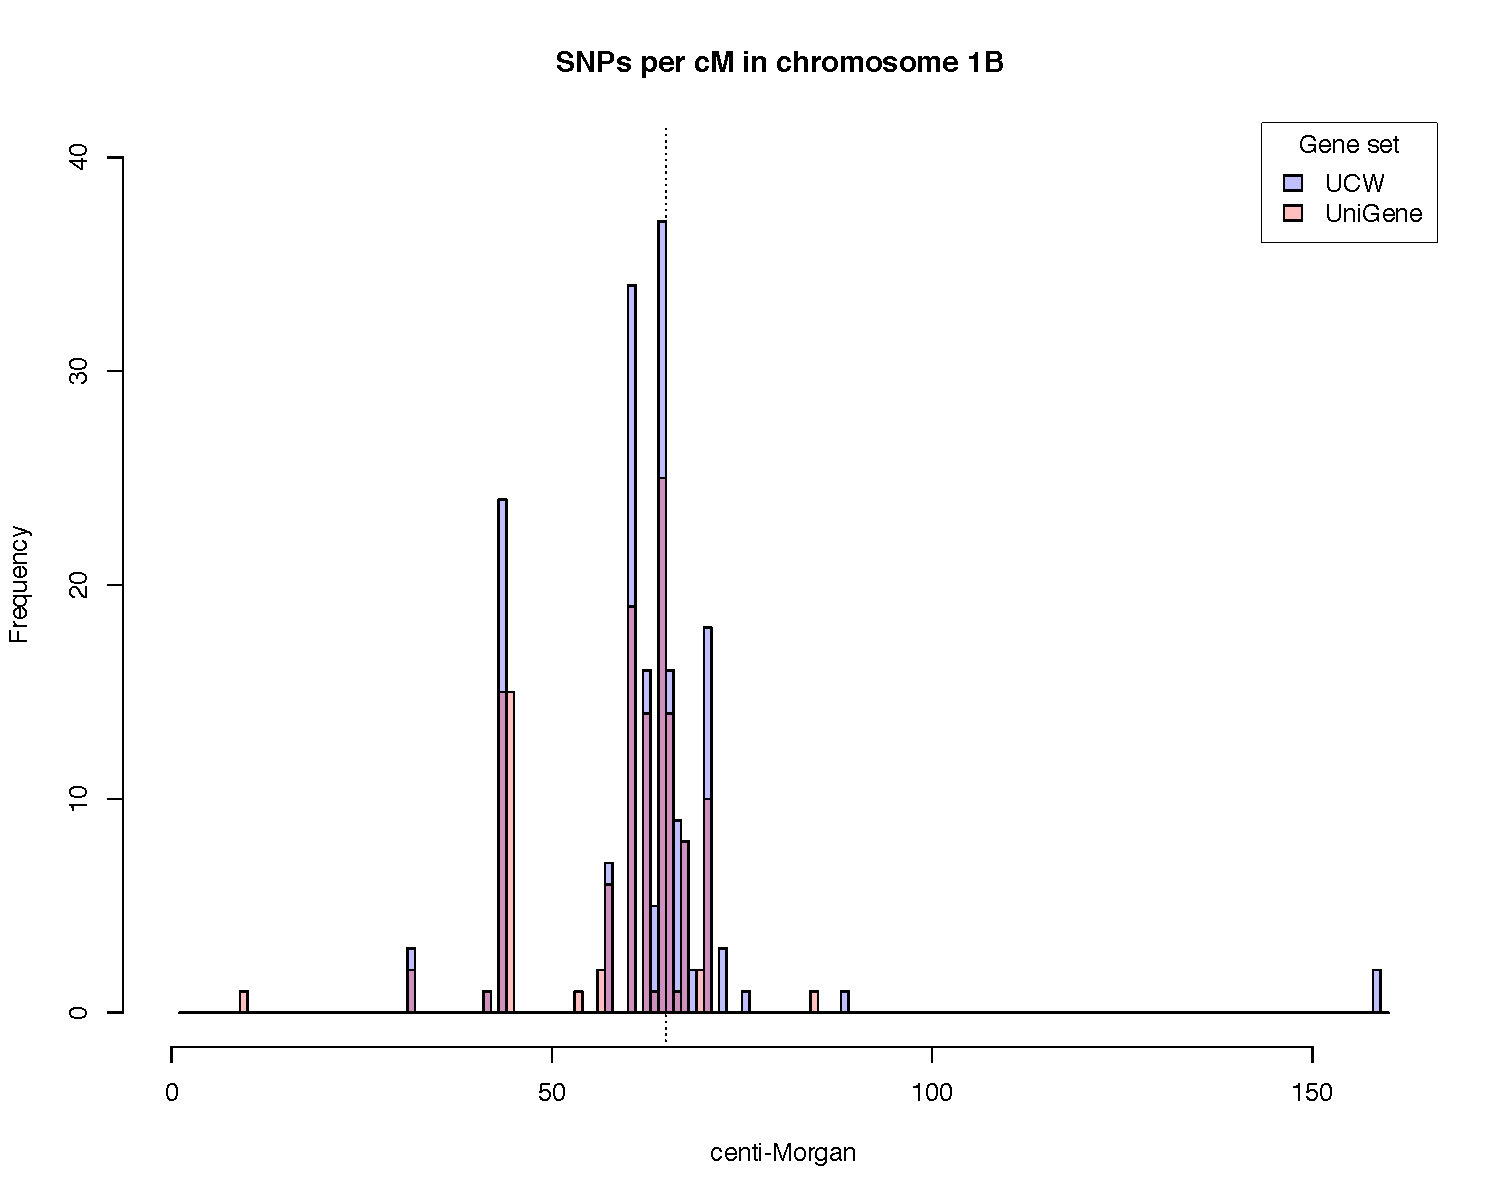
\includegraphics[width=1\textwidth]{Yr15/Figures/mapping/snpsBFR6crh1B.pdf}
  \end{subfigure}
  
  \begin{subfigure}{0.70\textwidth}
  \caption{}
   \label{fig:yr15:BFRValues1BS}
   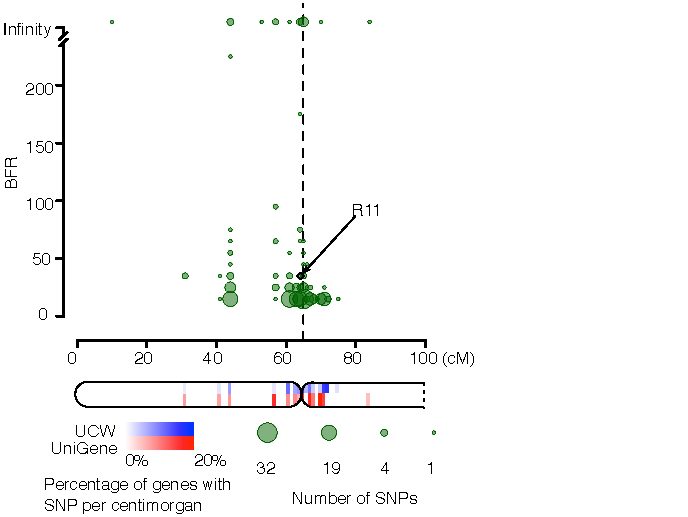
\includegraphics[width=1\textwidth]{Yr15/Figures/mapping/BFRValues1BS.pdf}
  \end{subfigure}
\caption[\textit{In silico} location of SNPs with BFR\textgreater6]{\textit{In silico} location of SNPs with $BFR>6$. (\subref{fig:yr15:snpsBFR6Chr1B}) Number of SNPs with $BFR>6$ per cM in chromosome 1B. (\subref{fig:yr15:BFRValues1BS}) BFRs of mapped genes with SNPs on chromosome 1B. The area of the circle represents the number of SNPs clustered by location (windows size: 10 cM) and BFR (window size: 5cM). R11 is the only marker near the \acrshort{yr15} locus that had a corresponding position in the genetic map. The percentage of genes with SNPs per cM is also illustrated based on UCW (blue) and UniGene (red) gene models. The centromere is imputed by the centre of a window of 10 cM where the short arm switches to the long in the genetic map. BFRs correspond to those from the mixed \textit{in silico} bulk S1 + S2 + S3/R1 + R2 + R3. Adapted from \citep{Ramirez-Gonzalez2015b}.} 
\label{fig:yr15:chr1}
\end{figure}

The \acrshort{css} assembly was used as a common reference between the reference genes and the 40,266 SNP markers published at the time \citep{Wang2014} to locate the SNPs with a $BFR>6$ (including $BFR=\infty$) in a genomic position (Figures \ref{fig:yr15:chr1}, \ref{fig:yr15:bfrs:0-6}).  
From the 1,582 SNPS across 1,173 genes,  only 678 SNPs ($43\%$, 474 genes) were successfully located in the genetic map. 
Since the \acrshort{css} assembly is quite fragmented, the low percentage of located SNPs can be because not all candidate SNPs had a corresponding scaffold that has at least one of the 40,266 markers in the genetic map. 
Even if the number of located SNPs was not enough to give a position for over $50\%$ of the SNPs from the parental line, the resolution of the genetic position SNPs that were assigned improved over just having the chromosome arm information from the CSS assembly. 
The mapping position further confirmed an enrichment of SNPs near the centromere of chromosome 1B with 325 out of 678 SNPs. 
Furthermore, 311 of those where located within an interval of 30cM (Figures \ref{fig:yr15:bfr6}, \ref{fig:yr15:snpsBFR6Chr1B}). 

Studies in diploid organisms using \acrshort{qtl}-Seq \citep{Takagi2013} or other \acrshort{ngs}-enabled genetic approaches \citep{James2013} have shown smooth curves with a defined peak in the region linked to the studied trait. 
In practice, we only observe clusters of SNPs with  enriched \acrshortpl{bfr} near the centromere of chromosome 1B (Figures \ref{fig:yr15:snpsBFR6Chr1B}, \ref{fig:yr15:bfr6}). 

\begin{figure}
	\centering
	\begin{subfigure}{0.4\textwidth}
	\caption{}
	\label{fig:yr15:bfr0}
	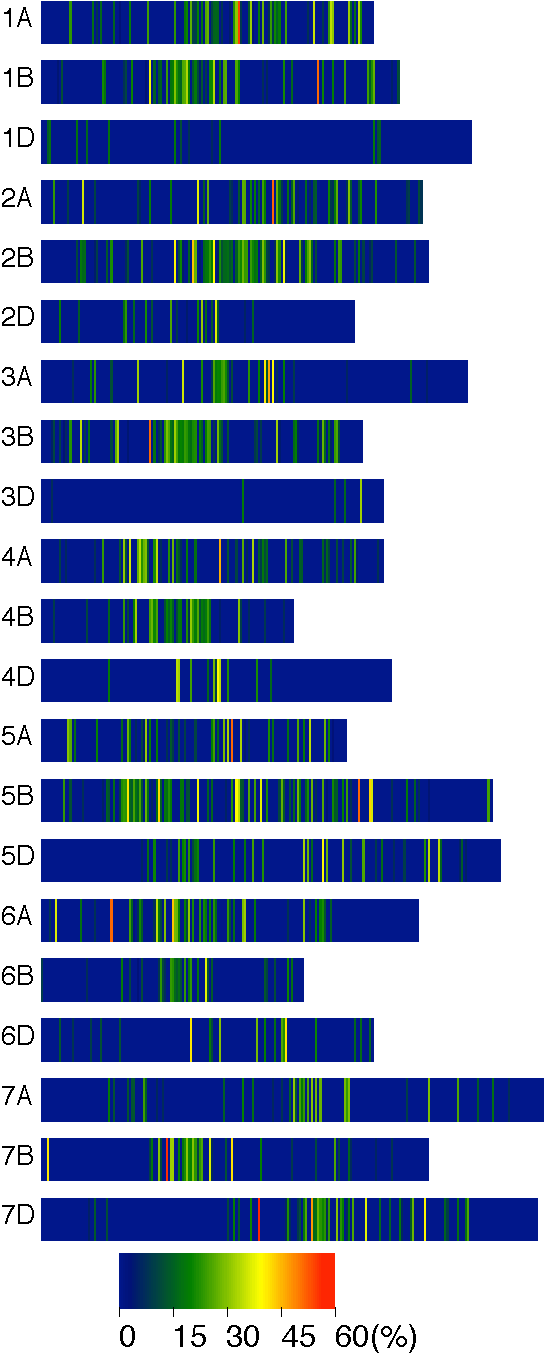
\includegraphics[height=0.55\textheight]{Yr15/Figures/mapping/snpsBFR0.pdf}
	\end{subfigure}
	~
	\begin{subfigure}{0.45\textwidth}
	\caption{}
	\label{fig:yr15:bfr6}
	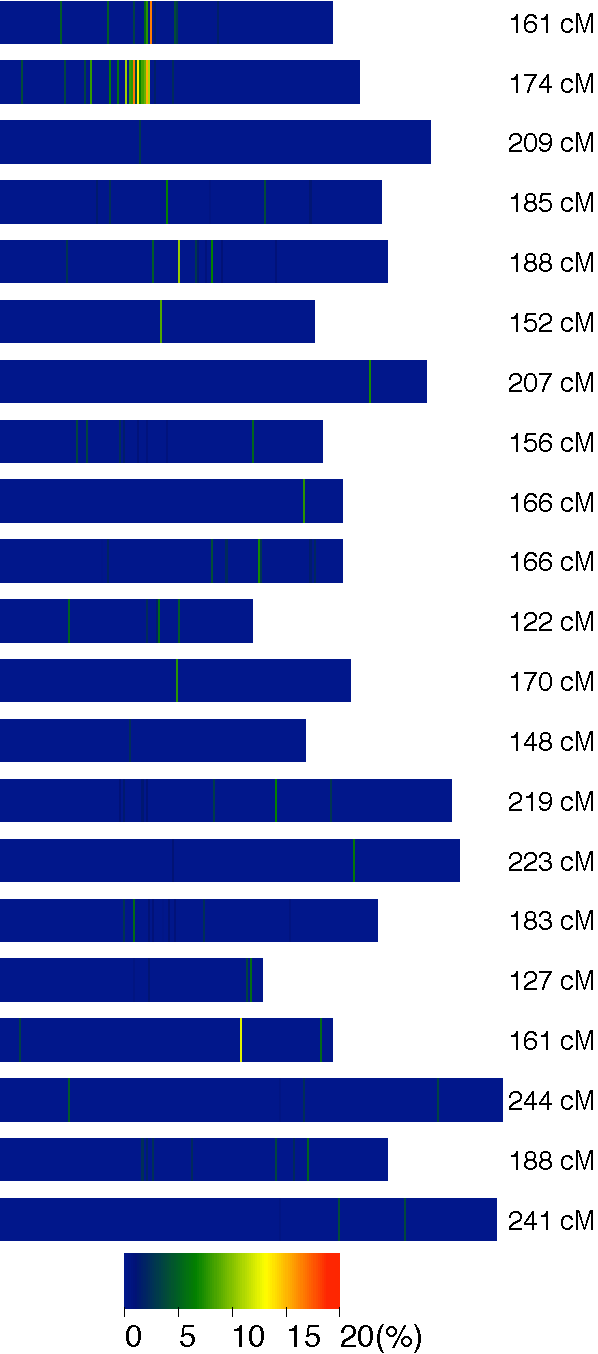
\includegraphics[height=0.55\textheight]{Yr15/Figures/mapping/snpsBFR6.pdf}
	\end{subfigure}
	\caption[Genetic location of genes with SNPs between AVS and Yr15.]{Genetic location of genes with SNPs between AVS and Yr15. The colour scale indicates the percentage of genes with SNPs per centi-Morgan (cM) across the 21 wheat chromosomes. The location of the genes was determined by the best alignment to the CSS scaffolds, and the location of these was determined by their position on a genetic map \citep{Wang2014} (\subref{fig:yr15:bfr0}). All the SNPs between progenitors. Note the lack of enrichment across any individual chromosome. (\subref{fig:yr15:bfr6}) SNPs with BFR$>$6. Note the enrichment in Chromosome 1B }
	\label{fig:yr15:bfrs:0-6}
\end{figure}

The location of the clusters with an enrichment of SNPs near the centromere is not expected on a random selection of genes, as the gene density increases with the distance to the centromere \citep{Akhunov2003}. 
This suggests that the experiment was successful on finding \acrshortpl{snp} linked to \acrshort{yr15}. 
There are several factor that prevent a clear peak; these include the biases induced by the differential expression and the fragmented reference sequence, with scaffolds that are not long enough to span genetic positions. 
Since there are several SNPs with a high BFR and the genetic map is not dense enough to locate a single region linked to \acrshort{yr15},  multiple criteria were needed to prioritise SNPs that were more likely to yield successful genetic markers.

\section{Assay selection} 
\label{yr15:assaySelection}
\begin{figure}
\centering
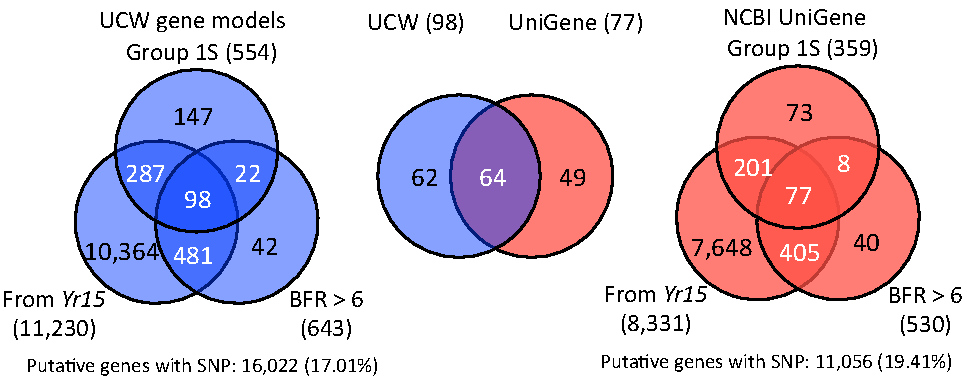
\includegraphics[width=1\textwidth]{Yr15/Figures/selection/snpSets.pdf}
\caption[Selection criteria for marker design]{Selection criteria for marker design. Venn diagrams based on the three selection criteria (SNP in the short arm of chromosome group 1; SNP has a $BFR>6$; and SNP is from the \acrshort{yr15} parent) for the UCW (blue) and UniGene (red) gene models. The centre diagram shows the intersection between common genes matching all three criteria across both data sets. Note that the numbers are not directly additive as in cases, multiple models from one reference set will relate to a single gene model in the other values. Published in \citep{Ramirez-Gonzalez2015b} }
\label{fig:yr15:snpset}
\end{figure}

Three independent criteria were used to prioritise the SNPs for marker development and validation: 

\begin{description}
\item[High BFR.] SNPs with a $BFR>6$ in at least two independent bulk replicates or in either of the \textit{in silico} mixes were selected to ensure consistency and recover SNPs with a low coverage on a particular bulk. 
\item[Group 1S.] SNPs that are in \acrshort{css} scaffolds in the short arm of chromosome group 1 were selected.
The selection included \glspl{snp} from the A, B and D genomes because the best hit to each gene model may be missing from the \gls{css} assembly.
Therefore, in cases where one or more of the homoeologous genes is missing from the reference, reads might be assigned to the wrong sub-genome.
This is consistent with the \textit{in silico} genetic map and with previous studies \citep{Murphy2009,Peng2000,Grama1997}.
\item[\acrshort{yr15} parent.] The SNPs should originate from the \acrshort{yr15} parent to ensure that the SNP is coming from the \textit{T. dicoccoides} introgression and not from a SNP in the \acrshort{avs} genetic background, who would be less useful in breeding programs with a different background.
\end{description}

Only SNPs meeting the three criteria were selected for further analysis. 

\begin{figure}
\centering
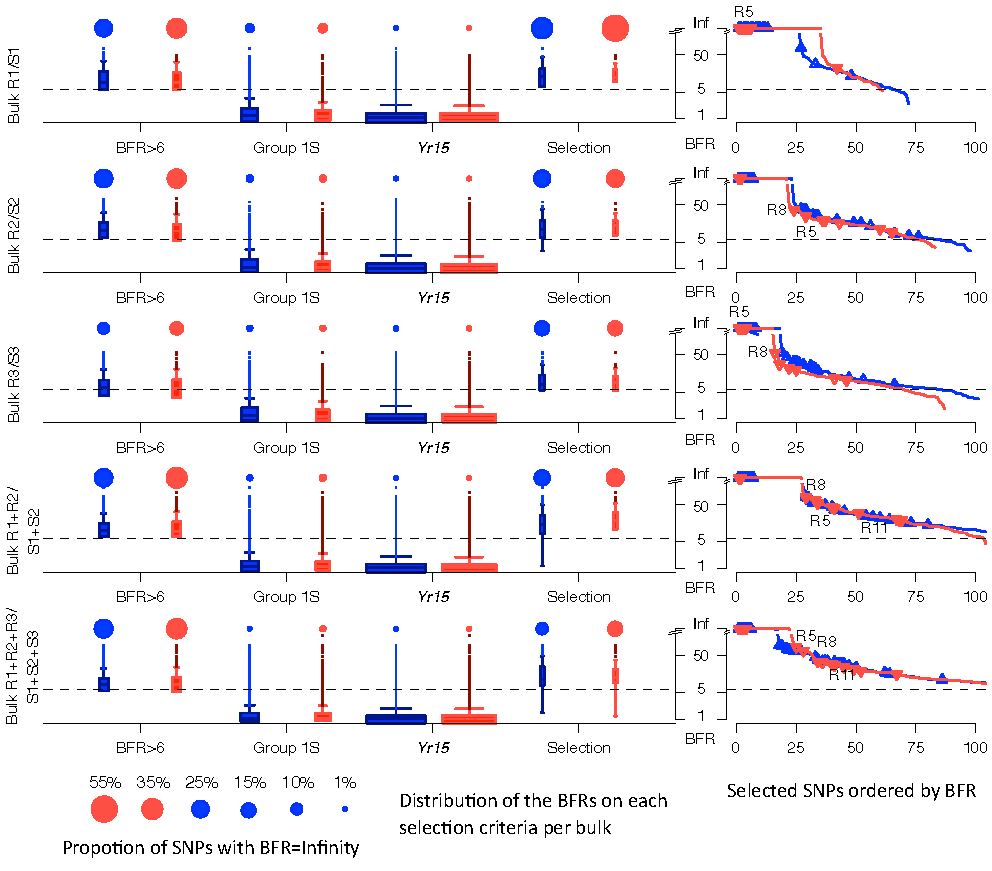
\includegraphics[width=1\textwidth]{Yr15/Figures/selection/selectionDetals.pdf}
\caption[BFRs of selected SNPs across bulks.]{BFRs of selected SNPs across the individual bulks and in silico mixes (UCW, red; UniGene, blue). The dotted line represents the BFR threshold of 6 (logarithmic scale). Left: Distribution of the BFRs for each selection criteria and the selected SNPs for validation. The circles on the top of each plot represent the percentage of SNPs with $BFR=\infty$. The Selection may include SNPs with $BFR<6$ when the same SNP has a higher score on the complementing reference (ie. $BFR>6$ on UCW, but $BFR<6$ on UniGenes). Right: The BFR values of selected SNPs were sorted in descending order across the different bulks and according to their origin. Validated SNPs are indicated by open triangles, and SNPs corresponding to markers R5, R8 and R11 are labelled across different bulks and mixes. Note that some SNPs are below the threshold in a specific bulk as they meet the BFR criteria across others. }
\label{fig:yr15:bfrDetailScore}
\end{figure}

Applying these multiple criteria, the number of genes with a putative SNP went down from over 27,000 to just 175; 77 and 98 from the UniGene and UCW gene sets, respectively.
As the two gene sets originate from independent sources, an overlap between the two selected sets is to be expected.
When we aligned the 77 and 98 genes from the two collections, we indeed found that around half of the genes overlap (Figure \ref{fig:yr15:snpset}). 
The 50 SNPs with the highest BFRs, out of the 175 genes, were selected for validation; fifteen of them were found to be redundant between references, resulting in a final set of 35 SNPs to validate. 

The separate bulks and the \textit{in silico} mixes were evaluated in detail to understand the behaviour and value of having multiple bulks. 
The initial expectation was that the number of SNPs with $BFR=\infty$ should drop in the mixes, as the improved coverage should reduce the number of instances where the absence of an allele is due to the lack of coverage on a particular sample. 
However, the opposite happened, the additional coverage in the \textit{in silico} mixes recovered SNPs in genes with a low expression at the time of the sampling (Figure \ref{fig:yr15:bfrDetailScore}).  
Some SNPs were present across all the samples, however the value of the BFR changed depending on the sample (e.g. marker R5). 
In some cases a \gls{snp} was missing in an individual bulk, but present in the rest and also in the mixes (e.g. marker R8). 
The main parameter affecting the scoring was the coverage in the sample for each particular gene, hence a strategy with a consistent coverage would be preferred for this kind of analysis.  
Previous studies have shown that a coverage of less than 5x is sufficient to call SNPs in model organisms with a high-quality reference \citep{Schneeberger2011}.
However, the results on this study are in line with other studies using populations for SNP calling \citep{Abe2012,Takagi2013}. 
The non-uniform distribution of the coverage in RNA-Seq experiments affects the number of reads that can be used to call for SNPs, especially on genes with a low expression level \citep{Mortazavi2008}. 

%!TEX root = ../../Main.tex
\begin{table}
\caption{ Number of genes (and SNPs) with a unique hit ($>99\%$ sequence identity) to a single wheat survey sequence scaffold. }
\label{tab:yr15:mappedGenes}
\centering
\begin{localsize}{9}{11}
\begin{tabular}{llrr@{\extracolsep{6pt}}rr@{\extracolsep{6pt}}rr}

\toprule
 \multicolumn{2}{l}{Chromosome 1}            &  \multicolumn{2}{c}{All SNPs} &  \multicolumn{2}{c}{BFR\ensuremath{>}6 }  &    \multicolumn{2}{c}{ \%  BFR\ensuremath{>}6 }       \\
  \cline{3-4}
  \cline{5-6}
  \cline{7-8}
                &            & SNP        & Genes  & SNP     & Genes  & SNPs               & Genes  \\
\midrule
 UCW            & Unique     & 5,283      & 1,245  & 311     & 214    & 5.89\%              & 17.19\% \\
                & Total      & 8,086      & 1,954  & 486     & 330    & 6.01\%              & 16.89\% \\
                & Percentage & 65.34\%     & 63.72\% & 63.99\%  & 64.85\% &                    &        \\
 \midrule
 UniGene        & Unique     & 3,687      & 745    & 213     & 139    & 5.78\%              & 18.66\% \\
                & Total      & 6,422      & 1,318  & 386     & 246    & 6.01\%              & 18.66\% \\
                & Percentage & 57.41\%     & 56.53\% & 49.17\%  & 56.07\% &                    &        \\
 \midrule
 UCW  & Unique     & 8,970      & 1,990  & 524     & 353    & 5.84\%              & 17.74\% \\
+              & Total      & 14,508     & 3,272  & 872     & 576    & 6.01\%              & 17.60\% \\
 UniGene       & Percentage & 61.83\%     & 60.82\% & 60.09\%  & 61.28\% &                    &        \\
\bottomrule
                &            &            &        &         &        &                    &        \\
\toprule
 All SNPs       &            &  \multicolumn{2}{c}{All SNPs} &  \multicolumn{2}{c}{BFR\ensuremath{>}6 }  &    \multicolumn{2}{c}{ \% BFR\ensuremath{>}6 }         \\
\cline{3-4}
\cline{5-6}
\cline{7-8}
                &            & SNP        & Genes  & SNP     & Genes  & SNPs               & Genes  \\
 \midrule
 UCW            & Unique     & 39,247     & 9,585  & 481     & 368    & 1.23\%              & 3.84\%  \\
                & Total      & 66,426     & 16,022 & 859     & 643    & 1.29\%              & 4.01\%  \\
                & Percentage & 59.08\%     & 59.82\% & 56.00\%  & 57.23\% &                    &        \\
 \midrule
 UniGene        & Unique     & 27,292     & 5,698  & 344     & 252    & 1.26\%              & 4.42\%  \\
                & Total      & 52,262     & 11,056 & 723     & 530    & 1.38\%              & 4.79\%  \\
                & Percentage & 52.22\%     & 51.54\% & 47.58\%  & 47.55\% &                    &        \\
 \midrule
 UCW  & Unique     & 66,539     & 15,283 & 825     & 620    & 1.24\%              & 4.06\%  \\
 +               & Total      & 118,688    & 27,078 & 1,582   & 1,173  & 1.33\%              & 4.33\%  \\
 UniGene       & Percentage & 56.06\%     & 56.44\% & 52.15\%  & 52.86\% &                    &        \\
\bottomrule
\end{tabular}
\end{localsize}
\end{table}


%TODO: maybe move to the discussion. 
Around $60\%$ of the gene models, across both references, had a unique hit with greater than 99\% sequence identity to a single \gls{css} scaffold (Table \ref{tab:yr15:mappedGenes}). 
%\unsure{This sentence is not completely clear.}
This is likely because the gene models don't have a unique mapping between gene sets because in cases where only one homoeologue is present in one reference, all the homoeologues in the complementary reference will map to the only represented gene in the original set of genes. 
To reduce the number of spurious SNPs we used IUPAC ambiguity codes (Section \ref{lit:ambiguity}, \citet{Cornish-Bowden1985}) when two different alleles were observed.
This had the side effect that in order to keep only high confidence SNPs we required a higher coverage ($>20x$). 
On the original study introducing the BFR in tetraploid wheat, the authors show that increasing the coverage, from $8x$ to $16x$, reduces the putative SNPs by $60\%$, but the validated SNPs increase from $57\%$ to $83\%$ \citep{Trick2012}. 
Hence, a compromise between increasing the minimum coverage at the cost of reducing the SNP candidates had to be reached in line with the objectives and available resources for this particular study. 

\section {SNP Validation}

KASP assays were designed to validate and generate a genetic map of the \acrshort{yr15} locus for the 35 selected SNPs.
To automate the design of genome-specific primers for polyploid organisms PolyMarker was developed (Chapter \ref{cha:polymarker}).
Out of the 35 assays to design, 17 were designed as specific, 9 as semi-specific to chromosome 1BS, and 9 were not specific because there was no information for the homoeologues on the \acrshort{css} scaffolds. 
PolyMarker also identified putative homoeologous variants (between genomes, as opposed to between varieties) that were in the list of candidate SNPs, but were not identified previously (Figure \ref{fig:poly:mask}; Table \ref{tab:yr15:polymarker}). 


\begin{figure}[b!]
\begin{subfigure}{0.31\textwidth}
\caption{}
\label{fig:yr15:r2}
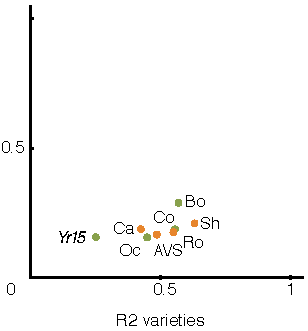
\includegraphics[width=1\textwidth]{Yr15/Figures/selection/R2.pdf}
\end{subfigure}
~
\begin{subfigure}{0.31\textwidth}
\caption{}
\label{fig:yr15:r8}
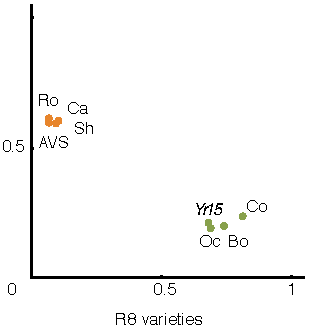
\includegraphics[width=1\textwidth]{Yr15/Figures/selection/R8.pdf}
\end{subfigure}
~
\begin{subfigure}{0.31\textwidth}
\caption{}
\label{fig:yr15:r8f2}
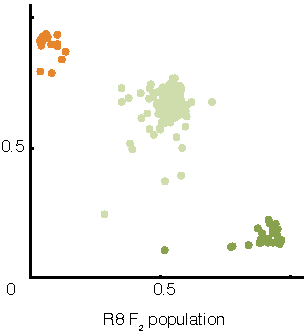
\includegraphics[width=1\textwidth]{Yr15/Figures/selection/R8F2.pdf}
\end{subfigure}

\caption[KASP output from the wheat variety panel]{KASP output from the wheat variety panel with (Ochre, Boston, Cortez) and without (Robigus, Cadenza and Shamrock) \acrshort{yr15}. Marker  R2 (\subref{fig:yr15:r2}) is monomorphic while R8 (\subref{fig:yr15:r8})  is polymorphic between varieties known to carry the gene.  Marker R8 results for the F2 population (\subref{fig:yr15:r8f2}) showing three distinct clusters. The central cluster (light green) is comprised of heterozygous individuals, whereas clusters near the axes are homozygous for either AVS (VIC; orange) or \acrshort{yr15} (FAM; dark green).}
\end{figure}


To validate if the 35 SNPs were polymorphic across the parents and diagnostic for \acrshort{yr15} we tested them in the progenitors plus six commercial varieties, three containing \acrshort{yr15} (Ochre, Boston and, Cortez) and three without it (Shamrock, Robigus and, Cadenza).
Two of the lines without \acrshort{yr15} have \textit{T. dicoccoides} in their pedigree (Shamrock and Robigus), as it is the donor species of \textit{Yr15} \citep{mcintosh1995}. 
This test panel allows to test if the SNPs are only diagnostic to \textit{T. dicoccoides} instead of \acrshort{yr15}.
On the test panel, 28 ($80\%$) SNPs were polymorphic across the parents and three of them where diagnostic to \textit{Yr15} (R5, R8, R33).
From the five homoeologous SNPs, three of them were monomorphic and two polymorphic, suggesting that PolyMarker is effective on detecting which assays are less likely to work (Table \ref{tab:yr15:markersToTest}; Figure \ref{fig:yr15:r2},\subref{fig:yr15:r8}).
The segregation of the SNPs in the full $F_{2}$ population (Section \ref{sub:mappingPopulation}, Figure \ref{fig:yr15:r8f2}) and a genetic map was produced (Section \ref{yr15:geneticMap}).   



%!TEX root = ../../Main.tex
\begin{sidewaystable}
\caption{Primer details for the markers to validate. }
\centering
\label{tab:yr15:polymarker}
\begin{localsize}{6}{9}

\begin{tabular}{lllllll}
\toprule
 Assay ID   & Polymorphism\_type   & AVS-specific primer         & Yr15-specific primer        & Common primer               & Specificity             & Orientation   \\
\midrule
 R1         & non-homeologous     & aactggtaatggtgcagCgG        & aactggtaatggtgcagCgC        & ttcaggataacacAggagatgtT     & chromosome\_semispecific & reverse       \\
 R2         & non-homeologous     & acatcaattcttcaggaaagctctaC  & acatcaattcttcaggaaagctctaT  & gcacagcttctcgtgttcTT        & chromosome\_specific     & forward       \\
 R3         & non-homeologous     & acgtggagaacctagattgcG       & acgtggagaacctagattgcC       & ccttttaggtgcgccaactT        & chromosome\_semispecific & reverse       \\
 R4         & non-homeologous     & agactctttgggcagtggatC       & agactctttgggcagtggatT       & cctcgggcgatctattctcT        & chromosome\_specific     & forward       \\
 R5         & non-homeologous     & agtcaacttggattacactgaagtT   & agtcaacttggattacactgaagtC   & agatatcacactgaacatactgatgaG & chromosome\_specific     & reverse       \\
 R6         & non-homeologous     & caagatgaagatgaagaggaatatgaT & caagatgaagatgaagaggaatatgaC & gCttgaccctgtaatcatactcG     & chromosome\_semispecific & forward       \\
 R7         & non-homeologous     & caccaccaTggaggccaC          & caccaccaTggaggccaT          & cgccgtggtagtgtccgG          & chromosome\_specific     & forward       \\
 R8         & non-homeologous     & cagatccccggttctctcaaG       & cagatccccggttctctcaaA       & cccccaaatgatcgagaata        & chromosome\_inspecific   & reverse       \\
 R9         & non-homeologous     & caggtgctgaaatgcatcC         & caggtgctgaaatgcatcT         & cggcctatcttcaggtctgt        & chromosome\_inspecific   & reverse       \\
 R10        & non-homeologous     & cattcgtcgcgccttctacG        & cattcgtcgcgccttctacA        & tcctaactcatatgcatgactcAC    & chromosome\_specific     & reverse       \\
 R11        & non-homeologous     & ccattctgatcaaggtcactgtcG    & ccattctgatcaaggtcactgtcA    & ttctgtaTggcaaCgggagC        & chromosome\_specific     & reverse       \\
 R12        & homeologous         & cttagccagtgaaccAggcC        & cttagccagtgaaccAggcT        & ggctgtttgttacCgtggaG        & chromosome\_specific     & reverse       \\
 R14        & non-homeologous     & gacTacAggtgcgatcccC         & gacTacAggtgcgatcccT         & ctcgcctgccagtcgTaT          & chromosome\_specific     & forward       \\
 R15        & homeologous         & gactagggctaccAttgttgA       & gactagggctaccAttgttgC       & agccctgCtaacaatggcaA        & chromosome\_specific     & reverse       \\
 R16        & non-homeologous     & gatgtaagcTAtgactggCgC       & gatgtaagcTAtgactggCgT       & tgcaactgatctttagcaggC       & chromosome\_semispecific & reverse       \\
 R17        & non-homeologous     & gcaAcaacaaCaaCaagtggT       & gcaAcaacaaCaaCaagtggC       & cctcaacctgcttgttgttgT       & chromosome\_specific     & forward       \\
 R19        & non-homeologous     & gcctgatttttaattcgctccaG     & gcctgatttttaattcgctccaA     & agagcactgatgatgacccC        & chromosome\_specific     & reverse       \\
 R20        & non-homeologous     & gctgtatcctcttgaaaaaggcT     & gctgtatcctcttgaaaaaggcC     & ttaggcatgtcagaaatgtagaaaa   & chromosome\_semispecific & forward       \\
 R21        & non-homeologous     & gcttcaaacatgccggctG         & gcttcaaacatgccggctT         & cggtctttttcaaccagggC        & chromosome\_semispecific & forward       \\
 R22        & homeologous         & gctTgtCttaaagccAtttccA      & gctTgtCttaaagccAtttccG      & gcctatcgttCgctaaactctaacT   & chromosome\_specific     & reverse       \\
 R23        & non-homeologous     & gctttaggcactatggattcAcC     & gctttaggcactatggattcAcT     & caggtttctgttcgacctcA        & chromosome\_specific     & forward       \\
 R24        & non-homeologous     & ggaggtcctacacgcgtctT        & ggaggtcctacacgcgtctG        & ctccaaaagaggggcatcattT      & chromosome\_semispecific & forward       \\
 R25        & non-homeologous     & gggttcctcacctgcgcC          & gggttcctcacctgcgcT          & ctctTtgcaatcggccagc         & chromosome\_inspecific   & reverse       \\
 R26        & non-homeologous     & gtCttcgcCggcacCacC          & gtCttcgcCggcacCacT          & agtggatcttgccgatctcg        & chromosome\_inspecific   & forward       \\
 R28        & non-homeologous     & tagatgagaccttggaCggA        & tagatgagaccttggaCggG        & cagtcatctaatgcggaacattcA    & chromosome\_semispecific & reverse       \\
 R29        & non-homeologous     & TatggtGtggccTtccccG         & TatggtGtggccTtccccA         & cgagctcgctgatgaacttG        & chromosome\_specific     & forward       \\
 R30        & non-homeologous     & tcagcagcccttttaacccaA       & tcagcagcccttttaacccaT       & agtaaatcgggcacggttgt        & chromosome\_inspecific   & reverse       \\
 R31        & homeologous         & tcatccatgtatatGaaTccaagcC   & tcatccatgtatatGaaTccaagcA   & tcacgcctgcaacAttcaaaT       & chromosome\_specific     & reverse       \\
 R32        & homeologous         & tccaatcttatggctttgcttctG    & tccaatcttatggctttgcttctT    & caggtgatgtagatgctgagaC      & chromosome\_semispecific & reverse       \\
 R33        & non-homeologous     & tccttcctgctatagctgaaagG     & tccttcctgctatagctgaaagT     & ccctttgcctgccatgtaga        & chromosome\_inspecific   & forward       \\
 R34        & non-homeologous     & tctgagatgatgatactTtgtggG    & tctgagatgatgatactTtgtggA    & actggggatgccctctgtat        & chromosome\_inspecific   & forward       \\
 R35        & non-homeologous     & tgaaagagtggaatttcttgttgT    & tgaaagagtggaatttcttgttgC    & ctttTagctgcttaattctattgcttC & chromosome\_specific     & forward       \\
 R36        & non-homeologous     & tgaaatgccttgtcaatgccA       & tgaaatgccttgtcaatgccG       & ATGCGAATTGGGGAATTAAA        & chromosome\_inspecific   & reverse       \\
 R37        & non-homeologous     & tgcatatgcctgaagagactcG      & tgcatatgcctgaagagactcA      & tgtccacctactcaagtctgc       & chromosome\_inspecific   & reverse       \\
 R38        & non-homeologous     & tgGcCaagTtTttctgcaagaT      & tgGcCaagTtTttctgcaagaG      & tgtaggaaggaactcCgaagtA      & chromosome\_specific     & forward       \\
 R40        & non-homeologous     & tgcatatgcctgaagagactcA      & tgcatatgcctgaagagactcG      & agtccgctaaagcattgcct        & chromosome\_nonspecific  & reverse       \\
 R43        & non-homeologous     & tcgctgatttcatcatgtcccA      & tcgctgatttcatcatgtcccG      & tcaggtgctgcaaatttgagG       & chromosome\_semispecific & forward       \\
\bottomrule
\end{tabular}
\end{localsize}
\end{sidewaystable}

%!TEX root = ../../Main.tex
\begin{sidewaystable}
\caption{Results of validation of primers on the progenitors (\acrshort{avs} and \acrshort{yr15}, varieties known to contain \acrshort{yr15} (Cortez, Ochre and, Boston) } and, varieties without \acrshort{yr15} (Robigus, Cadenza and, Shamrock). Shamrock and Robigus have \textit{T. dicoccoides} introgressions. The underlined markers are the diagnostic triplet. 

\label{tab:yr15:markersToTest}
\begin{localsize}{6}{9}
\centering
\begin{tabular}{llllllll|lllllll}
\toprule
Assay &             &                    &        & \begin{sideways}Yr15\end{sideways}    & \begin{sideways}Ochre\end{sideways}  & \begin{sideways}Boston\end{sideways}    & \begin{sideways}Cortez\end{sideways}    & \begin{sideways}Shamrock \end{sideways}    & \begin{sideways}Robigus\end{sideways}    & \begin{sideways}Cadenza\end{sideways}    & \begin{sideways}AVS\end{sideways} & \begin{sideways}Polymorphic\end{sideways} & \begin{sideways}Linked \acrshort{yr15}\end{sideways}  &\\
%\cline{5-8}
%\cline{9-12}
 ID   & Gene set    & Gene model name    & SNP    & \multicolumn{4}{c}{\acrshort{yr15}+ } & \multicolumn{4}{c}{\acrshort{yr15}- } &   &      & comment                 \\
\midrule
 R1         & UCW         & UCW\_Tt-k55\_contig\_8830;tt-k21\_contig\_10204                      & C341G  & A      & H         & A        & A        & A            & -         & A         & B     & Yes           & * &   segregation distortion                      \\
 R2         & UniGene v60 & gnl|UG|Ta\#S13126619                                             & C491T  & B      & B         & B        & B        & B            & B         & B         & B     & No            & -                      &                         \\
 R3         & UCW         & contig95240                                                     & C220G  & H      & B         & B        & B        & B            & B         & B         & B     & Yes           & Yes                    &                         \\
 R4         & UCW         & contig105384                                                    & C1227T & A      & B         & B        & B        & B            & B         & B         & B     & Yes           & Yes                    &                         \\
 R5         & UniGene v60 & gnl|UG|Ta\#S58861868                                             & A214G  & A      & A         & A        & A        & B            & B         & B         & B     & Yes           & Yes                    &                         \\
 \midrule
 R6         & UCW         & KukriC706\_1                                                     & T2979C & A      & H         & B        & B        & B            & B         & H         & H     & Yes           & No                     &                         \\
 R7         & UniGene v60 & gnl|UG|Ta\#S37932863                                             & C281T  & H      & A         & A        & A        & B            & B         & A         & B     & Yes           & No                     &                         \\
 R8         & UniGene v60 & gnl|UG|Ta\#S58863387                                             & T241C  & B      & B         & B        & B        & A            & A         & A         & A     & Yes           & Yes                    &                         \\
 \midrule
 R9         & UniGene v60 & gnl|UG|Ta\#S58892239                                             & C303T  & H      & B         & A        & B        & B            & B         & H         & B     & Yes           & No                     &                         \\
 R10        & UCW         & UCW\_Tt-k63\_contig\_79829                                         & C207T  & H      & A         & B        & A        & B            & B         & B         & B     & Yes           & Yes                    &                         \\

 R11        & UCW         & UCW\_Tt-k45\_contig\_39011                                         & C726T  & A      & A         & A        & H        & -            & B         & B         & B     & Yes           & Yes                    &                         \\
  \midrule
  R12        & UCW         & contig50308                                                     & G587A  & -      & H         & H        & H        & B            & B         & A         & B     & Yes           & Yes                    &                         \\
 R14        & UniGene v60 & gnl|UG|Ta\#S44692929                                             & C549T  & A      & A         & -        & A        & A            & B         & -         & B     & Yes           & Yes                    &                         \\
 R15        & UCW         & UCW\_Tt-k51\_contig\_2344;tt-k55\_contig\_2091                       & T686G  & A      & A         & A        & A        & A            & A         & A         & A     & No            & -                      &                         \\
 R16        & UniGene v60 & gnl|UG|Ta\#S17898149                                             & G227A  & A      & A         & B        & A        & B            & B         & B         & B     & Yes           & Yes                    &                         \\
 R17        & UCW         & CL3339Contig1                                                   & T509C  & H      & H         & H        & H        & H            & H         & H         & H     & No            & -                      &                         \\
 R19        & UCW         & UCW\_Tt-k21\_contig\_8407;tt-k61\_contig\_5972                       & C1405T & A      & B         & B        & B        & B            & B         & B         & B     & Yes           & Yes                    &                         \\
 R20        & UCW         & UCW\_Tt-k21\_contig\_8407;tt-k61\_contig\_5972                       & T1102C & A      & B         & B        & B        & -            & B         & B         & B     & Yes           & Yes                    &                         \\
 R21        & UCW         & UCW\_Tt-k31\_contig\_53804;tt-k41\_contig\_31582                     & G1810T & H      & B         & B        & B        & B            & B         & B         & B     & Yes           & Yes                    &                         \\
 R22        & UCW         & UCW\_Tt-k31\_contig\_14966                                         & T408C  & A      & A         & A        & A        & A            & A         & A         & B     & Yes           & Yes                    &                         \\
 R23        & UCW         & UCW\_Tt-k51\_contig\_12731;tt-k55\_contig\_13077;tt-k61\_contig\_18734 & C50T   & A      & H         & H        & H        & H            & -         & H         & B     & Yes           & Yes                    &                         \\
 R24        & UCW         & UCW\_Tt-k55\_contig\_8830;tt-k21\_contig\_10204                      & T3005G & H      & H         & B        & H        & B            & B         & B         & B     & Yes           & Yes                    &                         \\
 R25        & UCW         & UCW\_Tt-k63\_contig\_79829                                         & G184A  & A      & A         & A        & A        & H            & H         & A         & A     & No            & -                      &                         \\
 R26        & UCW         & UCW\_Tt-k21\_contig\_3794                                          & C702T  & H      & A         & B        & A        & B            & B         & B         & B     & Yes           & Yes                    &                         \\
 R28        & UCW         & KukriC3701\_1                                                    & T1053C & A      & A         & B        & A        & B            & B         & B         & B     & Yes           & Yes                    &                         \\
 R29        & UCW         & UCW\_Tt-k55\_contig\_8640;tt-k41\_contig\_8875                       & G783A  & H      & A         & B        & A        & B            & B         & B         & B     & Yes           & Yes                    &                         \\
 R30        & UCW         & UCW\_Tt-k55\_contig\_8830;tt-k21\_contig\_10204                      & T2184A & A      & A         & B        & A        & B            & B         & A         & B     & Yes           & Yes                    &                         \\
 R31        & UCW         & UCW\_Tt-k45\_contig\_22098                                         & G683T  & A      & B         & A        & B        & B            & B         & A         & B     & Yes           & Yes                    &                         \\
 R32        & UCW         & UCW\_Tt-k21\_contig\_33188;tt-k25\_contig\_30647                     & C596A  & H      & A         & A        & A        & A            & A         & A         & H     & No            & -                      &                         \\
 R33        & UniGene v60 & gnl|UG|Ta\#S58861868                                             & G486T  & A      & A         & A        & A        & B            & B         & B         & B     & Yes           & Yes                    &                         \\
 R34        & UCW         & UCW\_Tt-k31\_contig\_34099                                         & G1713A & H      & A         & B        & -        & B            & B         & B         & B     & Yes           & No                     &                         \\
 R35        & UniGene v60 & gnl|UG|Ta\#S58900202                                             & T889C  & A      & B         & B        & B        & B            & B         & B         & B     & Yes           & Yes                    &                         \\
 R36        & UCW         & UCW\_Tt-k55\_contig\_8830;tt-k21\_contig\_10204                      & T2349C & H      & H         & H        & H        & H            & -         & H         & B     & Yes           & Yes                    &                         \\
 R37        & UCW         & UCW\_Tt-k31\_contig\_34099                                         & C846T  & B      & B         & B        & B        & B            & B         & B         & B     & No            & -                      &                         \\
 R38        & UniGene v60 & gnl|UG|Ta\#S58840501                                             & T179G  & B      & B         & B        & B        & B            & B         & B         & B     & No            & -                      &                         \\
 R40        & UCW         & UCW\_Tt-k31\_contig\_34099                                         & C846T  & A      & H         & B        & A        & -            & B         & B         & B     & Yes           & No                     & based on barley synteny \\
 R43        & UniGene v60 & gnl|UG|Ta\#S58843705                                             & G268A  & A      & B         & B        & -        & -            & B         & -         & B     & Yes           & Yes                    & based on barley synteny \\
\bottomrule
\end{tabular}
\end{localsize}
\end{sidewaystable}


\section{Genetic map} 
\label{yr15:geneticMap}


Initially, the 28 polymorphic markers were used to genotype a subset of 66 plants from the $F_{2}$ population. 
From those, 23 (82\%) were linked to \acrshort{yr15} and several markers map in a small interval around \acrshort{yr15} (Figure \ref{fig:yr15:initialMap}; Table \ref{tab:yr15:markersToTest}), confirming that the multiple-criteria strategy(Section \ref{yr15:assaySelection}) for selecting candidate SNPs was effective. 
Then, the complete $F_{2}$ population was assessed with:
\begin{itemize}	
	\item  the seven markers that were most closely linked to \acrshort{yr15}, including two of the diagnostic markers from the variety panel (R5 and R8),
	\item The flanking \acrshort{ssr} microsatellite markers used by UK breeders for germoplasm selection (\textit{Xbarc8} and \textit{Xgwm413}).  These correspond to the best markers available to breeders at the time of the study.
	\item A marker based on barley-wheat synteny (R43) which met the selection criteria, but was not on the original set of 50 markers with high BFR. 
\end{itemize}

The $F_{2}$ population consisted on 232 plants with phenotypic information, of those 196 where genotyped reliably (no more than one data point missing). 
Using the eight SNP markers and 2 SRRs, the \acrshort{yr15} locus was mapped to an interval of 0.77cM, with R8/xgwm413 0.26cM distal, and R5/R11 0.77cM proximal from \acrshort{yr15} (Figure \ref{fig:yr15:finalMap},\subref{fig:yr15:mapDetails}). 


\begin{figure}
	\centering
	\begin{subfigure}{0.45\textwidth}
	\caption{}
	\label{fig:yr15:initialMap}
	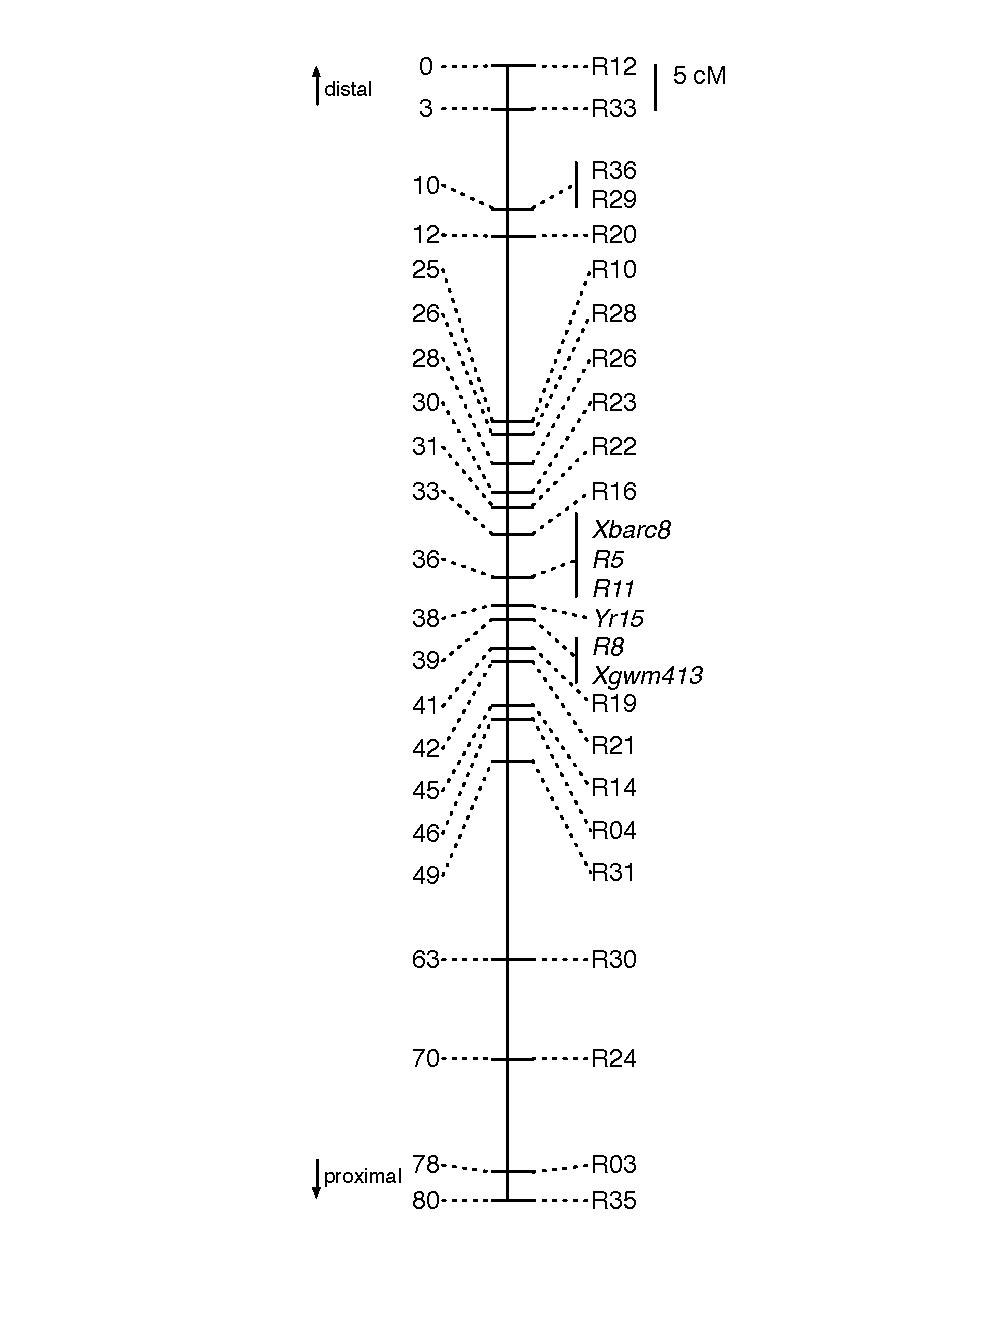
\includegraphics[height=0.45\textheight]{Yr15/Figures/selection/initialMap.pdf}
	\end{subfigure}
	~
	\begin{subfigure}{0.45\textwidth}
	\caption{}
	\label{fig:yr15:finalMap}
	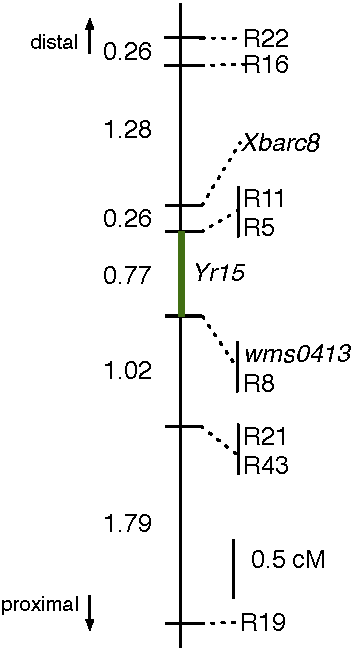
\includegraphics[height=0.45\textheight]{Yr15/Figures/selection/fineMap.pdf}
	\end{subfigure}

	\begin{subfigure}{1\textwidth}
	\caption{}
	\label{fig:yr15:mapDetails}
	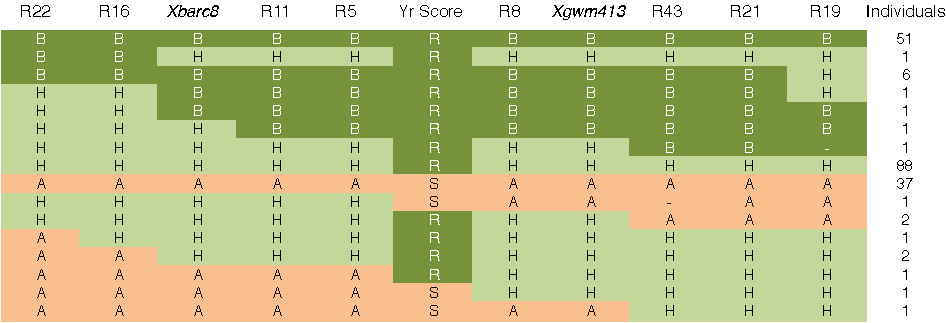
\includegraphics[width=1\textwidth]{Yr15/Figures/selection/mapDetails.pdf}
	\end{subfigure}
	

	\caption[Genetic maps for \acrshort{yr15}.]{Genetic maps for \acrshort{yr15}. (\subref{fig:yr15:initialMap}) Genetic map of the test panel from 50 individuals. (\subref{fig:yr15:finalMap}) Genetic map from 196 individuals from the full population only with the 8 markers previously identified as closer to the \acrshort{yr15} locus. (\subref{fig:yr15:mapDetails})Graphical genotype of the 196 $F_{2}$ individuals used to develop the genetic map. The alleles are abbreviated according to their origin: A: AVS; B: \textit{Yr15} and H: Heterozygous. Missing calls are indicated by a hyphen.}
\end{figure}

The sub-cM resolution is expected in a $F_{2}$ population of 196 individuals, as 392 gametes should provide n average resolution of 0.26cM. 
%\unsure{I assume here that mas pipelines prefer now to use SNPs.}
Despite the fact that none of the selected markers have perfect linkage to \gls{yr15}, the resulting genetic map is an improvement in the resolution of the map for the locus and it enables the shift to SNP markers from microsatellites. The former has become the preferred marker system in \gls{mas} pipelines in breeding programmes. 


\section{Methods}
\label{yr15:methods}

\begin{figure}
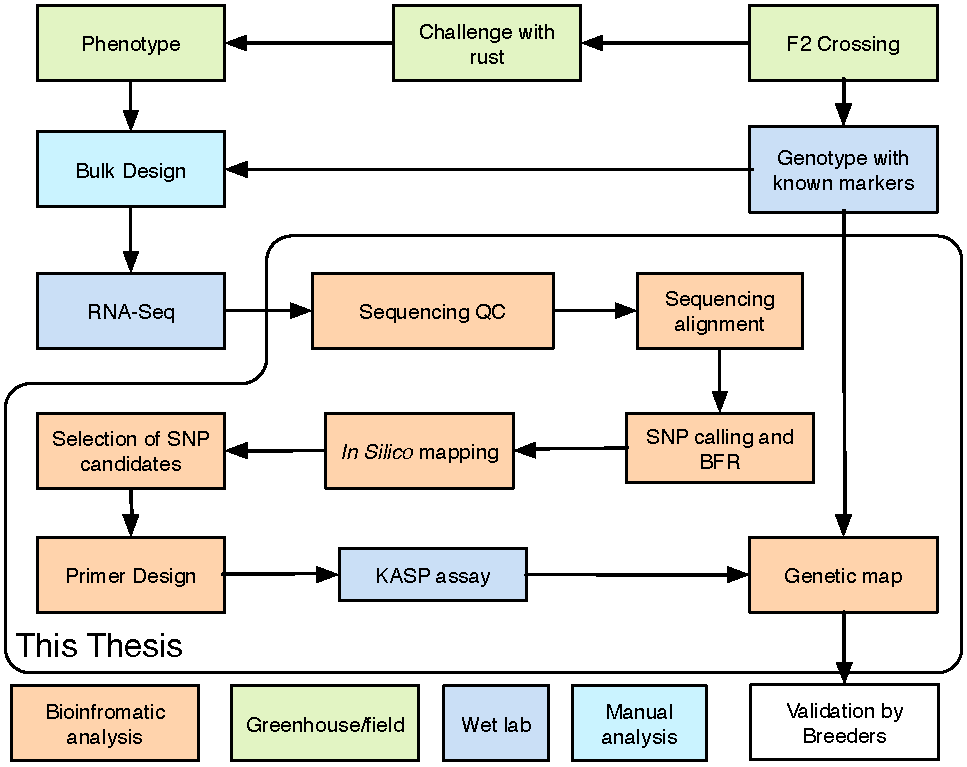
\includegraphics[width=1\textwidth]{Yr15/Figures/pipeline.pdf}
\caption{Steps used to go from the $F_{2}$ population to the genetic map.}
\end{figure}

The data analysis for this PhD required the use of some standard tools and custom developed code. 
All the code produced for this project is available and updated on the a github repository: \url{https://github.com/TGAC/bioruby-polyploid-tools}. 
For clarity, the snippets of code on this section had been simplified by removing the exception handling, type checks and caching mechanism.

\subsection{Base-call and Quality Control of sequencing reads}
The raw output from the Illumina HiSeq 2000 was processed with Casava v1.8 \citep{casavaBCL}. 
Lanes 1 and 2, containing multiplexed bulks (Table \ref{tab:yr15:reads}) was de-multiplexed with a tolerance of 1 mismatch in the barcode. 
Lanes 3 and 4 contained the parental sequences without a barcode. 
The FastQ files where left compressed and in chunks of 40,000, as the default for the BCL conversion pipeline from Casava to allow parallel processing in a cluster environment. 
The quality of the sequencing lanes was assessed with FastQC v0.10.1 \citep{fastqc}. 

\subsection{Alignment reads to gene models}
The RNA-Seq reads were aligned with BWA 0.5.9 \citep{Li2009} to the wheat UniGene database v60 \citep{PontiusJUWagnerL2002} and to the UCW gene models \citep{Krasileva2013}, including the \textit{T. turgidum} and complementary ORFs \citep{MASWheat2013}.
The alignments where sorted and stored as single BAM files to have random access \citep{Li2009a}. 
%\unsure{ Snippet with submission of the alignments. However I have not got access to the old cluster files.}


\subsection{Bulk Frequency Ratios and SNP calling}
\label{yr15:sub:bfr}
To avoid the creation of several temporary files with the coverage information on all the bases I developed a \texttt{Ruby} pipeline based on the \texttt{bio-samtools} library \citep{Ramirez-Gonzalez2012}, and some of the improvements to work with pileups were published as a follow-up on the library \citep{Etherington2015}.
To call for the consensus, the function \texttt{Bio::DB::Sam::mpileup} is called to generate the pileup of each gene. 
As the pileups are used several times during the analysis, a function that caches the current pileup is implemented.
The consensus is called by counting how many times each base appears, and if the number of bases is higher than \texttt{minumum\_ratio\_for\_iuap\_consensus} the base is added to the set of possible bases \citep{Cornish-Bowden1985} 
If there is no coverage at a certain position, the reference base is used, and set as lowercase. 
If the set of called bases is not empty, the ambiguity code for the observed bases is called, and set as upper case (Listing \ref{lst:yr15:consensus}).
The minimum ratio was done on 0.2 (20\%), as it allows calling for a consensus even when more than one homoeologue is mapping to the same reference.

\begin{code}[language=Ruby,caption=Method to call for the consensus on progenitors from a pileup, label=lst:yr15:consensus]
def consensus_iuap(minumum_ratio_for_iuap_consensus)
  minumum_ratio_for_iup_consensus
  @consensus_iuap = self.ref_base.downcase
  bases = self.bases
  tmp = String.new
  bases.each do |k,v|
    if v/self.coverage > minumum_ratio_for_iup_consensus
      tmp << k[0].to_s
    end 
    if tmp.length > 0
      @consensus_iuap = Bio::NucleicAcid.to_IUAPC(tmp)
    end
  end 
  @consensus_iuap.upcase
end
\end{code}

Then, to calculate the \acrshortpl{bfr} as shown on Figure \ref{fig:yr15:bfr} extra extensions for the \texttt{Bio::DB::Pileup} were added to get the actual number of bases in the pile (to exclude short insertions and deletions; Listing \ref{lst:yr15:cov}), and to calculate the SNP-Index (Listing \ref{lst:yr15:ratio}).  

\begin{code}[language=Ruby,caption=\texttt{base\_coverage} gets the number of bases called from a single pileup., label=lst:yr15:cov]
def base_coverage
  total = 0
  @bases.each do |k,v|
    total += v  
  end
  total
end
\end{code}

\begin{code}[language=Ruby,caption=\texttt{base\_ratios} gets the SNP-Index on a single pileup., label=lst:yr15:ratio]
def base_ratios
  return @base_ratios if @base_ratios
  bases = self.bases
  @base_ratios = Hash.new
  bases.each do |k,v| 
    @base_ratios[k] = v.to_f/self.base_coverage.to_f 
  end
  @base_ratios
 end
\end{code}

To calculate \acrshortpl{bfr} the class \texttt{Bio::BFRTools::Container} was implemented to contain all the \texttt{BIO:DB:Sam} objects corresponding to the progenitors and the bulks. 
The class \texttt{Bio::BFRTools::BFRRegion}  was implemented to contain the ratios and consensus sequences of each region. 
The method \texttt{bfr} uses the calculated SNP-Indices on every position, from the point of view of both progenitors (lines 15-16: Listing \ref{lst:yr15:bfr}, and in the case of lack of coverage the value is set to 0 or \texttt{Infinity} (lines 8-13), depending on the progenitor where the base is not called at all. 
Using this design where the values of each region are calculated at once reduces the number of times the pileup needs to be generated for each sample and allows to have in a single place in memory all the elements to calculate the \acrshortpl{bfr}, without having to write any temporary files on disc. 
Also, the fact that the calculation of each region is independent from that for other regions, it is possible to use a computing cluster to distribute the analysis on several nodes.

The code produces a table with the SNP-Indices and BFRs for all the SNPs found in the progenitors. 
The program was used to calculate the \glspl{bfr} on the independent conditions (Bulk 1: S1-R1, Bulk 2: S2-R2 and Bulk 3: S3-R3); the \textit{in silico} mixes of bulks 1 and 2; and bulks 1, 2 and 3. 


\begin{code}[language=Ruby,caption=Section of the code that , label=lst:yr15:bfr]
for i in (0..self.size-1)
  ratios_1 = @ratios_bulk_1[i]
  ratios_2 = @ratios_bulk_2[i]
  BASES.each do |base| 
    if ratios_1[base] == 0 and ratios_2[base] == 0
      bfr1 = 0
      bfr2 = 0
    elsif ratios_1[base] == 0
      bfr1 = 0
      bfr2 = Float::INFINITY
    elsif ratios_2[base] == 0
      bfr1 = Float::INFINITY
      bfr2 = 0
    else
      bfr1 = ratios_1[base] / ratios_2[base]
      bfr2 = ratios_2[base] / ratios_1[base]
    end
    @BFRs[:first][base] << bfr1
    @BFRs[:second][base] << bfr2
  end
end
\end{code}

\subsection{\textit{In Silico} mapping}
\label{yr15:met:inSilico}

To find the chromosomal position of the SNPs with a high BFR the sequences of the markers with a genetic position from \citet{Wang2014} were aligned with BLAT \citep{Kent2002} to the \acrshort{css} scaffolds \citep{Mayer2014}. 
The best hit for each query was found and cached using a \texttt{Ruby script}. 
Briefly, the class \texttt{Bio::Blat::Report} from \texttt{BioRuby} \citep{Goto2010} was extended to include an iterator only for the best alignment of each query: 
First, the whole file is iterated (line 5); the alignment with the best score is stored in a hash (lines 7-9) and finally the hash is iterated (line 11).
The script found 46,977 scaffolds that contained at least one marker from the map. 

\begin{code}[language=Ruby, caption={[\texttt{Bio::Blat::Report.each\_best\_hit}] Extension to \texttt{Bio::Blat::Report} that selects the best alignment from a \texttt{psl file from BLAT}}, label=lst:yr15:bestHit]
def self.each_best_hit(text = '')
  emptyHit = Bio::Blat::Report::Hit.new
  emptyHit.score = 0
  best_aln = Hash.new(emptyHit)
  self.each_hit(text) do |hit|
    current_score = hit.score
    if current_score > best_aln[current_name].score
      best_aln[current_name] = hit 
    end
  end
  best_aln.each_value { |val| yield  val }
end
\end{code}

Then, the UniGenes and the UCW gene models were also aligned with BLAT to the scaffolds that were located in the genetic map.  
The class \texttt{Bio::Blat::Report::Hit}  was extended to calculate how many bases are covered in the alignment and the percentage of covered bases in both, the target and query sequences (Listing \ref{lst:yr15:hit}).
Only the genes that align over 60\% of covered bases with an identity of at least 90\% were considered. 
This removes spurious mappings from repetitive regions, while retaining assignment to a homoeologue in the case in which the correct scaffold is not in the genetic map. 
The genes were also aligned to the full \acrshort{css} reference, to be able to allocate the genes to a chromosome arm, even when it is not possible to assign a position in neither the genetic map nor to the cDNAs of \textit{Hordeum vulgare} \citep{Mayer2011} (as deposited in Ensembl! Plants, release 16 \citep{Kersey2012}). 
%\unsure{Include code on how the coordinates where extracted, with the patch to the Ensembl package}
The genetic position of the contigs was used to calculate the density of SNPs between \acrshort{avs} and \acrshort{yr15} in the genetic bins for Figure \ref{fig:yr15:bfrs:0-6}. 
This information was used to select the SNPs with high BFR to validate.  

\begin{code}[language=Ruby, caption=Extension to \texttt{Bio::Blat::Report::Hit} for filtering of spurious alignments., label=lst:yr15:hit]
class Bio::Blat::Report::Hit
  def covered
    match + mismatch
  end
  def query_percentage_covered
    covered * 100.0 / query_len.to_f
  end
  def target_percentage_covered
    covered * 100.0 / target_len.to_f
  end
end
\end{code}

\subsection{Primer design and KASP assays}
The primer designs for KASP were designed with PolyMarker as described in Chapter \ref{cha:polymarker}. 
The only difference with default settings is that instead of using a template sequence, the sequence for each allele is calculated from the consensus of the alignments. 
As described in \citet{Ramirez-Gonzalez2015b}, 
\begin{blockquote} [the primers] were ordered from Sigma-Aldrich (Gillingham, UK), with primers carrying standard FAM or HEX compatible tails (FAM tail: 5' GAAGGTGACCAAGTTCATGCT 3'; HEX tail: 5' GAAGGTCGGAGTCAACGGATT 3') and the target SNP at the 30 end. 
Primer mix was set up as recommended by LGC [46 $\mu$L dH$_{2}$O, 30 $\mu$L common primer (100 $\mu$M) and 12 $\mu$L of each tailed primer (100 $\mu$M)] \citep{LGC}
Assays were tested in 384-well format and set up as 4-$\mu$L reactions [2-$\mu$L template (10–20 ng of DNA), 1.944 $\mu$L of V4 2 $\times$ Kaspar mix and 0.056 $\mu$L primer mix]. 
PCR cycling was performed on a Eppendorf Mastercycler pro 384 using the following protocol: hot-start at 95°C for 15 min, followed by ten touchdown cycles (95°C for 20s; touchdown 65°C, $-1$°C per cycle, 25 s) then followed by 30 cycles of amplification (95°C 10s; 57°C 60s).
As KASP amplicons are smaller than 120 bp, an extension step is unnecessary in the PCR protocol. 384-well optically clear plates (Cat. No. E10423000; Starlab Milton Keynes, UK) were read on a Tecan Safire plate reader. 
Fluorescence was detected at ambient temperature. If the signature genotyping clusters had not formed after the initial amplification, additional amplification cycles (usually 5–10) were conducted, and the samples were read again. Data analysis was performed manually using Klustercaller software (version 2.22.0.5; LGC Hoddesdon, UK).
\end{blockquote}


\subsection{Genetic map}
As described in \citet{Ramirez-Gonzalez2015b}:
\begin{blockquote}
 JoinMap version 3 \citep{vanOoijen2002} was used for linkage analysis and genetic map construction, using default settings. The linkage to \textit{Yr15} was determined using a divergent log-of-odds (LOD) threshold of 3.0, and genetic distances were computed based on recombination frequency. 
\end{blockquote}

\section{Discussion} 


Re-sequencing the $\sim17$Gbp genome of hexaploid wheat is costly and approaches to reduce the required sequenced volume to effectively call for SNPs had been evolving since the conception of this project. 
Both the RNA and DNA extraction and the sequencing for this project were carried out before the beginning of my PhD (before October 2012). 
At that time, exome capture was already an established technique for genotyping humans \citep{Ng2009}, however the first exome capture on wheat had just been published, with probes coming from unassembled 454 reads \citep{Winfield2012}; the first probe designed directly from transcripts \citep{Henry2014} was not published until after the analysis of this section was completed and validated (Figure \ref{fig:yr15:timeline}).
An even more targeted capture for resistance genes (RenSeq), by capturing genes with the NBS-LRR motif, was published while this study was executed \citep{Jupe2013}.
On the other hand, RNA-Seq had already been tested for \acrlong{bsa} on tetraploid wheat \citep{Trick2012}.  
Hence, the decision of reducing the sequenced space with RNA-Seq was appropriate at the time (Figure \ref{fig:yr15:timeline}). 
Unfortunately, one of the shortcomings of using RNA-Seq for calling SNPs is that the coverage is not uniform, and the genes that have low expression do not have enough coverage to allow reliable SNP calling (Section  \ref{yr15:sequencing}).
If a similar study had to be started today, a better alternative would be to use exome capture in general from a segregating population for any trait, or RenSeq if the target gene is a resistance gene. 

\begin{figure}
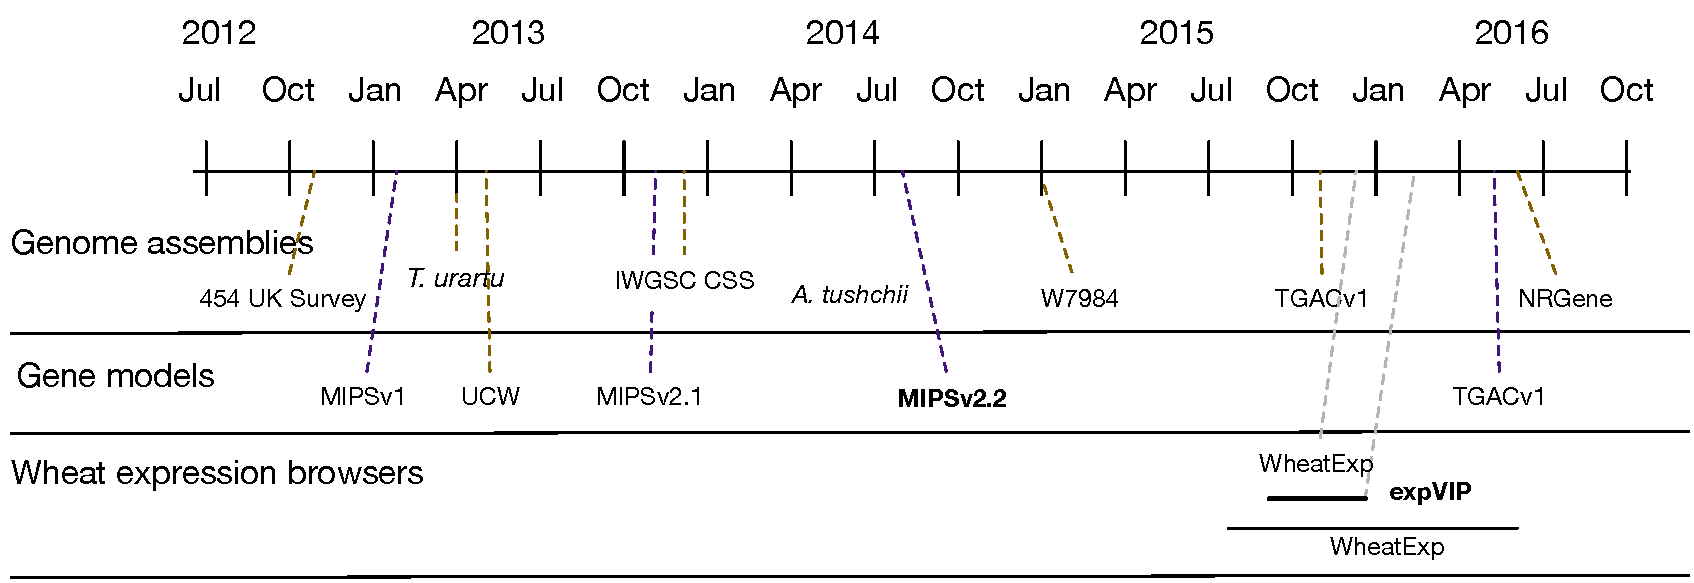
\includegraphics[width=1\textwidth]{expVIP/Figures/Timeline.pdf}
\caption{Timeline of resources used, or potentially used for \gls{yr15}.}
\label{fig:yr15:timeline}
\end{figure}

The quality and completeness  of the reference genome or gene models directly affects the mapping of \gls{ngs} reads. 
This is particularly true on polyploid organisms: if one of the homoeologues is absent, the reads are likely to map to the wrong genome if the parameters of the aligner are relaxed, or not map at all if the required identity is too high.
When the bioinformatic analysis of this project started, the only available wheat genomic reference was a whole genome shotgun 454 sequencing, unassembled \citep{Brenchley2012}; the \gls{css} assembly was being finished \citep{Mayer2014}; the longer scaffolds from \citet{Chapman2015} were not public yet; and finally, the efforts to make a whole genome shotgun assembly were being planned independently by the International Wheat Genome Sequencing consortium  \citep{Pozniak2016} and TGAC (\citealt{Clavijo2016} ; Figure \ref{fig:yr15:timeline}).  
Because a contiguous assembly with the corresponding annotation was not available at the time of the analysis, and the fact that all the data available was derived from transcriptomic sequencing, the use of gene models as a reference for the alignment was a suitable approach. 

In terms of available gene sets when the analysis started, the canonical reference was the UniGenes from the NCBI \citep{PontiusJUWagnerL2002}. 
The UniGenes are produced with an automated pipeline that clusters all the \glspl{est} deposited in the NCBI by identity and selects the longest transcript, which can merge homoeologous transcripts as a single reference.
Shortly after I started the bioinformatic analysis, two additional gene models were made available, the draft annotation for the \gls{css} assembly (MIPSv1) in January 2013 and the UCW gene models \citep{Krasileva2013} in May 2013. 
I selected the UCW gene models, as they were more mature, phased to distinguish between genomes and already published, over the MIPSv1 genes, as they were still being refined from an initial approach of lifting proteins from related organisms combined with few RNA-Seq experiments.  
The MIPS gene models were improved by removing duplications in the assembly in a later stage and the nomenclature before the release of the assembly \citep{Mayer2014}, but at that point the results of this project had already been submitted for publication (Figure \ref{fig:intro:timeline}; \citealt{Ramirez-Gonzalez2015b}). 
 
To locate the gene models in the chromosome arms and see if there was an enrichment on the called SNPs, the use of a high resolution consensus map is needed, as the genome assemblies available during the analysis are fragmented. 
Initially, I used barley to locate the gene models because the genetic map used to locate the \gls{css} scaffolds was not released yet and barley has a conserved synteny across the wheat genomes. 
The release of a genetic map with over 42,000 markers \citep{Wang2014} was extremely timely, as it happened during the last phase of the project.
Furthermore, as I collaborated in the project, I was also able to use it to locate several \acrshort{css} scaffolds before the release of the assembly. 
The located scaffolds were used as proxy to sort just under half of the reference genes in their chromosomal position (Section \ref{sub:yr15:inSilico}). 
Despite the resolution not being enough to find a single point of enrichment, it was enough to confirm that the SNPs were in the expected location, including one of the SNP candidates flanking the \textit{Yr15} locus (SNP R11, Figure \ref{fig:yr15:BFRValues1BS}).  
If the analysis was to be done today, the genetic map from \citet{Chapman2015} along with their longer scaffolds, or the scaffolds from TGACv1 or the NRGene should provide a better resolution. 
Even without having all the \acrshort{css} scaffolds sorted, the fact that they come from individual chromosome arms enabled the assignment of the genes to a chromosome. 

The original expectation was to have a \gls{nil} for the \gls{bsa} to simplify the SNP discovery and analysis since the majority, if indeed not all of the SNPs should be restricted to the region immediately flanking Yr15. However the number of \glspl{snp} called in the progenitors suggested that the background, \acrlong{avs}, was not the same.  
This happened because despite both susceptible lines being called the same and having the same response to the pathogen, they are in fact different lines from different countries (Section \ref{yr15:snpCalling}). 
This highlights the importance of genotyping the material used when developing mapping populations, especially if the seeds come from different seed banks. 

Despite these shortcomings, the use of the \glspl{bfr} to score the putative SNPs was effective, as most of the SNPs with a high score  mapped in chromosome 1B, in line with previous studies ($BFR>6$, Section \ref{yr15:assaySelection}).
Using the extra criteria of only selecting SNPs from the resistant progenitor and in the expected chromosome arm, I was able to produce a high resolution genetic map (Section \ref{yr15:geneticMap}). 
The genetic map was of the expected resolution for the size of the population (0.26cM on 196 individuals).
Since the mapping population contained only one critical recombinant between \textit{Yr15} and the flanking markers, the population could not yield a better map. 
To improve the map, a cross from the two critical recombinants could be used to repeat a similar analysis, sequencing with either exome capture or RenSeq. 
%\unsure{Talk about Why is R33 diagnostic on the varieties, but maps away?. }

\begin{figure}
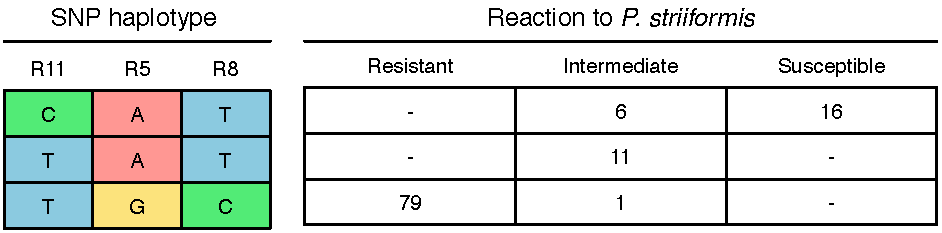
\includegraphics[width=1\textwidth]{Yr15/Figures/breedersTest.pdf}
\caption[Haplotype and phenotype of 113 doubled haploid lines]{Haplotype analysis and phenotypic evaluation of the 113 doubled haploid lines used in the study. The TGC haplotype corresponds to that originally identified in the \textit{Yr15} parent and which was diagnostic across 112 of the 113 lines studied. Figure from \citep{Ramirez-Gonzalez2015b}}
\label{fig:yr15:breeders}
\end{figure}

As described in \citet{Ramirez-Gonzalez2015b}:  
\begin{blockquote} The markers
 R11, R5 and R8 were tested across 122 doubled haploid (DH) lines. 
These DH lines were derived from crosses crosses between five different UK varieties/breeding lines to \textit{Yr15} derivatives known to carry the resistance gene. 
The expected \textit{Yr15} haplotype corresponded to T, G and C alleles at markers R11, R5 and R8, respectively (TGC haplotype). 
The DH lines were tested at seedling stage for reaction to \textit{P. striiformis}, with 84 showing complete resistance and 34 presenting an intermediate or completely susceptible reaction.
The resistant lines all carried the complete \textit{Yr15} haplotype (TGC, Figure \ref{fig:yr15:breeders}) across the three SNP markers with the exception of five lines which had a single missing data point, but were otherwise consistent. 
This compared favourably with the most diagnostic in-house SNP markers available within the breeding programmes. 
Using the three in-house markers, 79 resistant lines carried the expected haplotype, but five completely resistant DH lines were scored as false negative due to the presence of the non-\textit{Yr15} haplotype. 
Within the intermediate and susceptible DH lines, all but one had a non-\textit{Yr15} haplotype (CAT or TAT) across R11, R5 and R8 (Figure \ref{fig:yr15:breeders}). This single DH line was scored as a false positive as it carried the TGC \textit{Yr15} haplotype, but was found to have an intermediate (chlorotic) reaction to \textit{P. striiformis}. This line was also the only one scored as a false positive using the three in-house markers.
\end{blockquote}
%\unsure{This is a very long quote, but I'm finding hard to shorten it. } 
The fact that the developed markers perform better than markers developed by breeders shows the value of this particular experiment and further confirms that \gls{bsa} combined with \gls{ngs} is an effective way to develop novel markers. 
%\unsure{ Mention other people using a similar strategy since this was published. }

%TODO: Discuss other people using the mark 

In this chapter the integration of different levels of data helped to improve the selection of the candidate SNPs. 
The main criteria for selecting \glspl{snp}  was the \gls{bfr} score.
Thanks to the genetic map from \citet{Wang2014} and the \gls{css} scaffolds from \citet{Mayer2014}, we were able to confirm that the high scoring \glspl{snp} were in the expected region. 
As the reference genome for wheat improves, defining the location of SNPs linked to a trait of interest will become easier. 
With a continuous reference between two markers flanking a locus and an improved annotation, it will also be possible to compile a more focused set of candidate genes.
